\documentclass{article}

\PassOptionsToPackage{numbers, compress}{natbib}
\usepackage{neurips_2026}
% \usepackage[final,main]{neurips_2026}

\usepackage[utf8]{inputenc} % allow utf-8 input
\usepackage[T1]{fontenc}    % use 8-bit T1 fonts
\usepackage{hyperref}       % hyperlinks
\usepackage{url}            % simple URL typesetting
\usepackage{booktabs}       % professional-quality tables
\usepackage{amsfonts}       % blackboard math symbols
\usepackage{amsmath}        % math environments
\usepackage{amssymb}        % math symbols
\usepackage{amsthm}         % theorem environments (proof, etc.)
\usepackage{nicefrac}       % compact symbols for 1/2, etc.
\usepackage{microtype}      % microtypography
\usepackage{xcolor}         % colors
\usepackage{graphicx}       % figures
\usepackage{algorithm}      % algorithm environment
\usepackage{algorithmic}    % algorithmic pseudocode
\usepackage{multirow}       % multi-row tables
\usepackage{subcaption}     % subfigures
\usepackage{float}          % [H] float specifier
\usepackage{tikz}           % diagrams
\usetikzlibrary{arrows.meta, positioning, calc, fit, backgrounds, decorations.pathreplacing}
\usepackage{placeins}       % \FloatBarrier to keep figures within their section

% Tighter float spacing for page-budget compression
\setlength{\textfloatsep}{8pt plus 1pt minus 2pt}
\setlength{\intextsep}{8pt plus 1pt minus 2pt}
\setlength{\floatsep}{8pt plus 1pt minus 2pt}
\setlength{\dbltextfloatsep}{8pt plus 1pt minus 2pt}
\setlength{\abovecaptionskip}{4pt}
\setlength{\belowcaptionskip}{0pt}

% Theorem environments
\newtheorem{assumption}{Assumption}
\newtheorem{proposition}{Proposition}

% Custom math commands
\newcommand{\loss}{\mathcal{L}}
\newcommand{\encoder}{f}
\newcommand{\probe}{h}
\newcommand{\modality}[1]{\mathcal{M}_{#1}}
\newcommand{\boostscale}[1]{\alpha_{#1}}
\newcommand{\sg}{\operatorname{sg}}

% \title{Probe-Guided Gradient Boosting for Balanced Multimodal Learning}
\title{Probe-Guided Gradient Balancing for Multimodal Learning}


\author{%
  Vo Quoc Vu \\
  School of Science, Engineering \& Technology \\
  RMIT University \\
  \texttt{s3575819@rmit.edu.vn} \\
  \And
  Haytham Fayek \\
  School of Science, Engineering \& Technology \\
  RMIT University \\
  \texttt{haytham.fayek@rmit.edu.au} \\
  \And
  Thuy Nguyen \\
  School of Science, Engineering \& Technology \\
  RMIT University \\
  \texttt{thuy.nguyen43@rmit.edu.vn} \\
}


\begin{document}


\maketitle


\begin{abstract}

Jointly trained multimodal networks frequently underutilize their weaker modalities, as faster-learning modalities dominate the shared fusion objective and suppress the gradient signal reaching slower ones. Most existing approaches throttle the dominant modality, whereas directly boosting the weaker modality often fails because monitoring signals derived from the joint loss are entangled with, and thus dominated by, the stronger modality.
We propose a new gradient modulation approach, probe-guided gradient boosting (PGGB), to address the problem by probing and boosting the weak modalities while preserving the strength of the dominant modality. 
Probing is performed by attaching a lightweight linear classifier to each modality’s stop-gradient features to estimate the corresponding representation quality score. The conditionally unbiased gap between these scores across modalities, the \emph{utilization gap}, serves as an imbalance signal that defines a bounded and smoothed scaling factor adaptively reweighing the gradients of weaker modalities, enabling stable and effective rebalancing during joint optimization.
The method is composable with throttling methods as the intervention leaves the loss and fusion architecture unchanged. 
Extensive experiments were conducted across eight benchmarks spanning four domains and 2–4 modalities. The results show that our method outperforms state-of-the-art approaches on highly imbalanced multimodal datasets, while remaining competitive on benchmarks with low or no modality imbalance.
Bounded scaling, self-attenuation, and a standard-SGD descent bound were established under standard smoothness and bounded-variance assumptions. 
\end{abstract}

%=============================================================================
% SECTION 1: INTRODUCTION
%=============================================================================
\section{Introduction}
\label{sec:intro}

% --- P1: Multimodal learning is important and powerful ---
% Hook: Multimodal systems combine complementary information from different sensory channels.
% Theoretical promise: provably better than any single modality under reasonable assumptions.
% Cite: Huang et al. NeurIPS 2021 (provable multimodal superiority), Baltrušaitis survey
% Keep this brief — 3-4 sentences max.

% --- P2: The modality imbalance problem ---
% Introduce the "greedy modality" / "modality laziness" phenomenon.
% In late-fusion networks, the dominant modality converges faster and captures the shared
% classification head. The weaker modality's gradient signal is suppressed.
% This is widely observed: audio dominates visual in CREMA-D, text dominates in sentiment.
% Cite: wang2020gblending (first empirical identification), peng2022ogmge (OGM-GE)
% 3-4 sentences.

Multimodal learning integrates complementary signals across heterogeneous sources, including audio, visual, and textual streams among others~\citep{baltrusaitis2019multimodal}. Under mild assumptions on latent structure, multimodal models are provably superior to their unimodal counterparts~\citep{huang2021multimodal}. Despite this theoretical promise, jointly trained multimodal networks frequently fail to fully exploit all available modalities, often performing no better than their strongest unimodal component. This \emph{modality laziness} effect~\citep{wang2020gblending,peng2022ogmge,du2023suppression} has been observed for instance in audio-dominant emotion recognition on CREMA-D~\citep{cao2014cremad}.

% --- P3: State-of-the-art + Gap (4 sentences) ---
% Many methods exist, dominated by throttling paradigm.
% Key limitation: boosting the weak fails with coupled monitoring.

Existing methods share a \emph{throttle-only orientation}, intervening primarily by damping the dominant modality's gradient~\citep{peng2022ogmge,wei2024mmpareto,guo2024cggm,wei2024opm,fan2023pmr,kontras2024mlgm}. Some include nominally bidirectional terms~\citep{li2023agm,gao2025arm,huang2025inforeg,wei2025improving}, but throttling empirically dominates, and \citet{wei2024opm}'s symmetric boost-direction variant fails to close the gap. In late-fusion, every encoder's gradient flows through a shared classifier whose loss-derivative is dominated by the strong modality's contribution to the fusion loss. Amplifying the weak encoder's gradient therefore rescales an already-corrupted shared signal. Recent methods take partial steps~\citep{yang2025iprm,jiang2025aug} but continue to monitor imbalance through signals coupled to the joint training objective.

% --- P4: Proposed method (high-level, 4 sentences) ---
% Probe-guided gradient boosting with decoupled monitoring.
% Composable with existing throttling methods.
% No implementation details (save for Section 3).

We propose \emph{probe-guided gradient boosting} (PGGB): lightweight linear probes~\citep{alain2017understanding} on stop-gradient features (the stop-gradient operator passes activations forward but blocks the gradient at the backward pass~\citep{vandenoord2017vqvae}) yield a per-modality representation-quality estimate, whose cross-modality spread defines the \emph{utilization gap}, independent of the shared classifier's loss-derivative, removing the chain-rule coupling that impaired prior boost-the-weak attempts~\citep{wei2024opm}. The signal drives a bounded multiplicative factor on the weaker encoder's gradient, smoothed by an exponential moving average (EMA)~\citep{tarvainen2017mean} with a hard cap and gap-driven decay toward identity. Because the factor acts only on encoder gradients and modifies neither the loss nor the fusion architecture, it is \emph{composable} with throttling methods, multiplying with their suppression factors to produce two-sided pressure toward balance.

% --- P5: Main results (3 sentences) ---
% Experiments on 6 datasets. Key quantitative results.

We evaluate PGGB on eight benchmarks spanning audio-visual, sentiment, text-image, and medical-segmentation tasks (details in Section~\ref{sec:datasets}). The main gain is observed on the high-imbalance CREMA-D benchmark (3-frame), where composing PGGB with a representative gradient-modulation baseline~\citep{peng2022ogmge} reaches $71.45 \pm 1.71\%$ accuracy, $+2.31$~pp over the same baseline alone and $+9.86$~pp over joint training. On low-imbalance benchmarks, PGGB alone is the best-performing method on four of five low-imbalance datasets (Table~\ref{tab:main_results}). MOSI is the only low-imbalance dataset where PGGB alone trails the strongest baseline ($-0.79$~pp). The OGM-GE composition variant has two isolated regressions versus joint training (Kinetics-Sounds $-1.72$~pp, Sarcasm $-0.64$~pp) noted in Section~\ref{sec:conclusion}, while several gradient-modulation baselines degrade on multiple datasets (e.g., this baseline~\citep{peng2022ogmge} regresses on Kinetics-Sounds by $-1.80$~pp, Table~\ref{tab:main_results}).

% --- Contributions (4 bullets) ---
\paragraph{Contributions.}
\begin{itemize}
    \item We identify a \emph{throttle-only bias} in the modality-balancing literature and show that its natural complement, boosting the weaker modality, fails when the monitoring signal is coupled to the joint training objective via shared loss derivatives in late fusion.

    \item We propose \emph{decoupled probe monitoring}, a diagnostic attaching lightweight linear probes to stop-gradient features, yielding a conditionally unbiased \emph{utilization gap} estimate (the spread of per-modality probe accuracies) independent of the joint objective. The decoupling enables effective weak-modality boosting where prior coupled-monitoring boost-the-weak attempts failed~\citep{wei2024opm}.

    \item We introduce \emph{PGGB}, one instantiation that converts the monitor signal into a bounded multiplicative scaling on the weaker encoder's gradients. It is composable with existing throttling methods (Appendix~\ref{app:composability} validates non-destructive composition with four such methods).

    \item We validate \emph{PGGB} on eight benchmarks spanning audio-visual, sentiment, text-image, and medical-segmentation tasks. \emph{PGGB} composed with throttling outperforms state-of-the-art baselines on high-imbalance audio-visual (CREMA-D) and matches the strongest available baseline on medical segmentation (BraTS~2021, $+0.28$~pp, within seed variance), and \emph{PGGB} used alone is the best-performing method on four of five low-imbalance datasets and within seed variance on MOSI.
\end{itemize}


%=============================================================================
% SECTION 2: RELATED WORK
%=============================================================================
\section{Related work}
\label{sec:related}

% --- 2.1: Modality imbalance in joint training ---
\paragraph{Modality imbalance in joint training.}
% The phenomenon: jointly trained multimodal networks underperform the best unimodal
% component. First observed empirically by Wang et al. (G-Blending, CVPR 2020).
% Theoretical foundations:
%   - Huang et al. ICML 2022: proved only a subset of modalities are learned;
%     exact calculations for unimodal phase duration under Gaussian mixture model.
%   - Du et al. ICML 2023: feature suppression analysis.
%   - Zhang et al. ICML 2024: architecture/init-dependent unimodal phase in deep linear nets.
% Connect to "modality laziness" / "greedy modality" terminology.
% Cite: wang2020gblending, huang2022modality, du2023suppression, zhang2024unimodal
% 4-5 sentences.

Jointly trained multimodal networks frequently underperform their best unimodal component~\citep{wang2020gblending}. Under a Gaussian mixture model, \citet{huang2022modality} prove that joint training learns only a subset of modalities and derive bounds on the duration of the resulting unimodal phase, and \citet{du2023suppression} characterize the conditions under which individual modality features fail to be learned. \citet{zhang2024unimodal} further show, in deep linear networks, that this unimodal phase depends on architecture depth and initialization. Modality imbalance is therefore a structural property of joint optimization, rooted in the shared loss through which all encoder gradients flow.


% --- 2.2: Gradient modulation methods (throttle-dominant paradigm) ---
\paragraph{Gradient modulation for modality balance.}
% The dominant approach: modify gradient magnitudes/directions during backpropagation.
% Organize chronologically:
%   - GradNorm (Chen et al. ICML 2018): normalize gradient magnitudes across tasks.
%   - PCGrad (Yu et al. NeurIPS 2020): project conflicting gradients.
%   - OGM-GE (Peng et al. CVPR 2022 Oral): throttle dominant via discriminative ratio + noise.
%   - AGM (Li et al. ICCV 2023): Shapley-value gradient modulation — claims both boost/throttle.
%   - CGGM (Guo et al. NeurIPS 2024): coupled auxiliary classifiers for magnitude + direction.
%   - MLGM (Kontras et al. BMVC 2024): multi-loss gradient modulation with acceleration.
%   - GMML (ACM MM 2025): l2-norm constraints with convergence guarantees.
% KEY POINT for us: overwhelmingly throttle-dominant. Even CGGM/AGM that claim bidirectional
% are dominated by the throttling term. OGM* (Wei et al. TPAMI 2024) explicitly showed
% that boost-weak-only fails under coupled monitoring.
% Cite: chen2018gradnorm, yu2020pcgrad, peng2022ogmge, li2023agm, guo2024cggm, kontras2024mlgm
% 5-6 sentences.

The dominant response has been to modulate gradient magnitudes during backpropagation. Multi-task precursors GradNorm~\citep{chen2018gradnorm} and PCGrad~\citep{yu2020pcgrad} inspired a line of multimodal work. OGM-GE~\citep{peng2022ogmge} damps the dominant modality's gradient via a ratio of per-modality contributions to the target-class score, refined by AGM~\citep{li2023agm}, CGGM~\citep{guo2024cggm}, and MLGM~\citep{kontras2024mlgm}. Although some methods include bidirectional terms, throttling empirically dominates and boost-only variants remain ineffective: the symmetric boost direction (OGM*) reported in~\citet{peng2022ogmge} fails to close the modality gap, which we attribute to coupled monitoring signals affected by the dominant modality (Section~\ref{sec:method}). M-SAM~\citep{nowdeh2025msam} pairs Shapley attribution with sharpness-aware perturbation, inheriting the same coupled-monitoring limitation.


% --- 2.3: Beyond gradient modulation ---
\paragraph{Alternative approaches to modality balance.}
% Methods that go beyond gradient scaling:
%   - OPM (Wei et al. TPAMI 2024): feed-forward feature dropping for dominant modality.
%   - ARL (Wei et al. ICCV 2025): bias-variance framework, inverse-variance weighting.
%   - MMPareto (ICML 2024): Pareto optimization resolving gradient conflicts.
%   - ReconBoost (Hua et al. ICML 2024): modality-alternating training + KL reconcilement.
%   - MLA (Zhang et al. CVPR 2024): alternating unimodal adaptation + entropy fusion.
%   - D&R (Wei et al. ECCV 2024): representation separability diagnosis + reinitialization.
%   - InfoReg (Huang et al. CVPR 2025): Fisher information regulation during prime window.
%   - ARM (Gao et al. AAAI 2025): conditional mutual information for asymmetric reinforcement.
%   - MSLR (Yao & Mihalcea ACL 2022): modality-specific learning rates.
%   - Data Remixing (Ma et al. ICML 2025): data decoupling and reassembly.
% KEY POINT: diverse interventions (loss, architecture, data, learning rate) but all use
% coupled monitoring — gradient ratio, loss contribution, or live-model predictions.
% Cite: wei2024opm, wei2025improving, wei2024mmpareto, hua2024reconboost, zhang2024mla,
%       wei2024dr, huang2025inforeg, gao2025arm, yao2022mslr
% 5-6 sentences.

Beyond gradient scaling, a broader set of interventions has been proposed. These include feed-forward feature modulation~\citep{wei2024opm} and Pareto-optimal aggregation~\citep{wei2024mmpareto}. Modality-alternating schemes interleave unimodal and joint updates~\citep{hua2024reconboost,zhang2024mla}. Diagnostic methods detect imbalance through separability~\citep{wei2024dr}, Fisher information~\citep{huang2025inforeg}, or bias-variance decomposition~\citep{wei2025improving}. Other approaches intervene at the data or learning-rate level~\citep{yao2022mslr,guerra2025miles,ma2025remixing,yu2026tcmax}. Despite their diversity, these methods share a common design choice. Imbalance is detected through signals \emph{coupled} to the joint objective, such as gradient ratios, per-modality losses, or live-model predictions (with the partial exception of PMR's decoupled unimodal prototypes~\citep{fan2023pmr}). These are precisely the quantities distorted by dominant-modality dynamics, which limits the reliability of the resulting corrections.


% --- 2.4: Probing and monitoring in multimodal learning ---
\paragraph{Representation monitoring and probing.}
% Linear probes as evaluation tools: Alain & Bengio 2017 (understanding intermediate layers).
% Widely used in self-supervised learning (SimCLR, BYOL) to assess representation quality.
% In multimodal context:
%   - IPRM (Yang et al. IJCAI 2025): two-pass probe-and-rebalance, but probes are COUPLED
%     (use live-model predictions via KL divergence, not detached features).
%   - AUG (Jiang et al. NeurIPS 2025): loss-based detection of weak modality — coupled.
%   - PMR (Fan et al. CVPR 2023): prototype-based decoupled unimodal evaluation.
%   - CGGM: coupled auxiliary classifiers participate in the loss.
% KEY POINT: no existing method combines (1) truly decoupled probes (detached features,
% separate optimizers) with (2) gradient-level boosting of the weak modality.
% Our split-batch evaluation (train on first half, evaluate on second) further prevents
% probe overfitting — a protocol not used in any prior work.
% Cite: alain2017understanding, yang2025iprm, jiang2025aug, fan2023pmr, guo2024cggm
% 5-6 sentences. This is where we set up our method's unique position.

Linear probes on frozen representations~\citep{alain2017understanding} are a standard tool for assessing representation quality. Several multimodal methods adopt probe-like monitoring but retain coupling to the joint objective. IPRM's two-pass forward strategy compares unimodal and fused predictions of the live model via KL divergence~\citep{yang2025iprm}, CGGM's auxiliary classifiers participate in the training loss~\citep{guo2024cggm}, and AUG~\citep{jiang2025aug} relies on loss-based weakness signals that inherit the dominant modality's bias. PMR~\citep{fan2023pmr} moves toward decoupling via unimodal prototypes but the prototype signal feeds a gradient coefficient on the shared encoder, while DI-MML~\citep{fan2024dimml} detaches only the unimodal pre-fusion stage. In contrast, we train \emph{fully decoupled} linear probes on stop-gradient features with separate optimizers and evaluate them on held-out within-batch samples to prevent probe overfitting. The resulting utilization gap directly boosts the weaker encoder's gradients, so the imbalance estimate is not affected by the dynamics it aims to correct.


%=============================================================================
% SECTION 3: METHOD
%=============================================================================
\section{Probe-Guided Gradient Boosting}
\label{sec:method}

We present PGGB in four stages: problem formulation (\S\ref{sec:problem}), decoupled probe monitoring (\S\ref{sec:probes}), the boost mechanism (\S\ref{sec:boost}), and composability with existing balancing methods (\S\ref{sec:compose}). Algorithm~\ref{alg:pgb} summarizes the complete training procedure. Figure~\ref{fig:architecture} traces the data flow: the top row depicts the forward path (\S\ref{sec:problem}), the dashed bottom row depicts probe monitoring on stop-gradient features (\S\ref{sec:probes}), and the green boost block plus actuation rail depict the gradient-modification mechanism (\S\ref{sec:boost}). Composition with throttling (\S\ref{sec:compose}) is described in text only.

%---------- 3.1 Problem Formulation ----------
\subsection{Problem formulation}
\label{sec:problem}

Each multimodal sample comprises $M$ inputs $\{\mathbf{x}_m\}_{m=1}^{M}$, one per modality. Encoder $\encoder_m$ with parameters $\theta_m$ maps $\mathbf{x}_m$ to $\mathbf{z}_m$:
%
\begin{equation}
\label{eq:encoder}
\mathbf{z}_m = \encoder_m(\mathbf{x}_m;\,\theta_m) \in \mathbb{R}^d.
\end{equation}
%
Each $\mathbf{z}_m$ is a $d$-dimensional real vector with $d$ common across modalities. The features are concatenated and passed through a fusion classifier $g$ parameterized by $\phi$, yielding the prediction $\hat{y} = g([\mathbf{z}_1;\ldots;\mathbf{z}_M];\,\phi)$. With ground-truth label $y$, training minimizes the cross-entropy loss:
%
\begin{equation}
\label{eq:joint_loss}
\loss_{\text{fusion}} = \mathrm{CE}\!\bigl(\hat{y},\; y\bigr).
\end{equation}
%
By the chain rule, the gradient with respect to encoder parameters decomposes as
%
\begin{equation}
\label{eq:gradient_chain}
{\partial \loss_{\text{fusion}}}/{\partial \theta_m} = ({\partial \loss_{\text{fusion}}}/{\partial g})\,({\partial g}/{\partial \mathbf{z}_m})\,({\partial \mathbf{z}_m}/{\partial \theta_m}).
\end{equation}
%
The term ${\partial \loss_{\text{fusion}}}/{\partial g}$ is shared across all modalities, since all encoder outputs flow through the same fusion classifier. This shared dependency is the root of coupled monitoring failure: when one modality (say $m{=}1$) converges faster and begins to dominate the classifier's predictions, ${\partial \loss_{\text{fusion}}}/{\partial g}$ increasingly reflects the dominant modality's contribution. Any monitoring signal derived from $\loss_{\text{fusion}}$ or its gradients, including the discrepancy ratio used by OGM-GE~\citep{peng2022ogmge} and the auxiliary classifier losses used by CGGM~\citep{guo2024cggm}, inherits this bias.


%---------- Figure 1: Architecture overview (rendered from figures/architecture.tex) ----------
\begin{figure}[t]
\centering
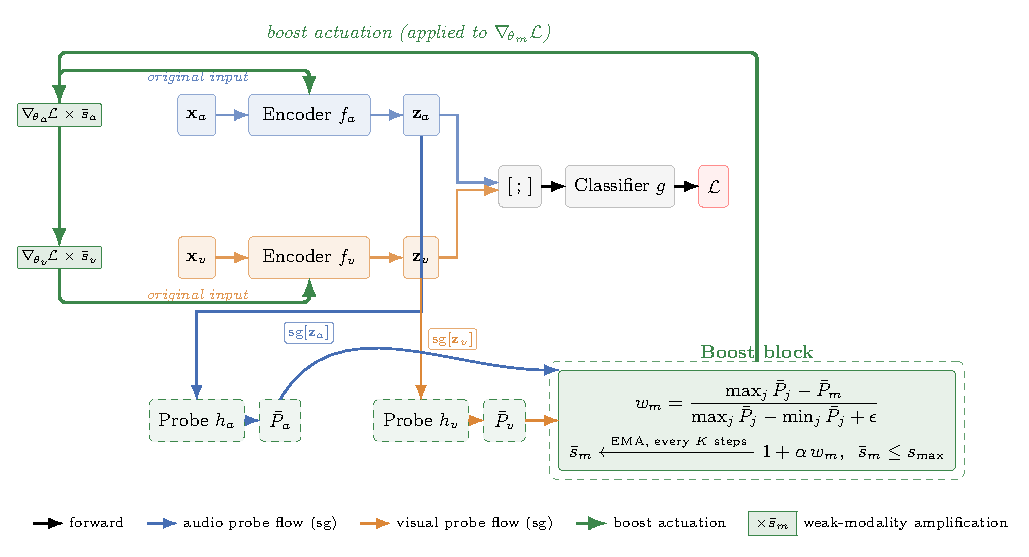
\includegraphics[width=0.95\textwidth]{figures/architecture.pdf}
\caption{Illustration of probe-guided gradient boosting on 2 modalities. \textbf{Top row:} encoder features $\mathbf{z}_m$ are concatenated and classified via the shared fusion classifier $g$, producing $\loss$. \textbf{Bottom row:} stop-gradient features $\sg[\mathbf{z}_m]$ are evaluated by linear probes (dashed green), yielding per-modality accuracies $\bar{P}_m$. The boost block computes the relative-gap weight $w_m$, an EMA-smoothed scale $\bar{s}_m$ refreshed only at probe-evaluation events (every $K$ steps, held constant in between), and clips it at $s_{\max}$. The actuation rail (thick green) applies $\bar{s}_m$ to the per-modality gradient $\nabla_{\!\theta_m}\loss$ before the optimizer step. Probes never backpropagate into encoders, so the monitoring signal is structurally decoupled from the fusion objective.}
\label{fig:architecture}
\end{figure}


%---------- 3.2 Decoupled Probe Monitoring ----------
\FloatBarrier
\subsection{Decoupled probe monitoring}
\label{sec:probes}

We attach a lightweight linear probe $\probe_m\colon \mathbb{R}^d \to \mathbb{R}^C$ (with $C$ classes) to each encoder, parameterized by $\psi_m$. The resulting probe accuracies define an imbalance signal, the \emph{utilization gap} (Eq.~\ref{eq:utilization_gap}), independent of the joint training objective. The probes are trained on stop-gradient features $\sg[\mathbf{z}_m]$, where $\sg[\cdot]$ denotes the stop-gradient operator~\citep{vandenoord2017vqvae} (identity at the forward pass, zero partial derivatives at the backward pass):
%
\begin{equation}
\label{eq:probe_loss}
\loss_{\text{probe},m} = \mathrm{CE}\!\bigl(\probe_m(\sg[\mathbf{z}_m];\,\psi_m),\; y\bigr).
\end{equation}
%
Each probe has its own optimizer that updates only $\psi_m$, and no gradient flows into $\theta_m$. Since $\sg[\mathbf{z}_m]$ halts backward propagation at the feature level, $\loss_{\text{probe},m}$ depends only on the quality of $\mathbf{z}_m$ as a representation, not on how it contributes through $g$. This is precisely why decoupling matters: the probe accuracy $P_m$ measures representation quality not influenced by the dominant modality's influence on $g$.

\paragraph{Split-batch evaluation and on-the-fly estimation.}
Every $K$ training iteration (we use $K{=}20$), we partition the (shuffled) mini-batch into two disjoint halves, training probes on the first half and evaluating on the second. This yields a \emph{conditionally unbiased} estimate $P_m$ of the current probe's training-distribution accuracy (conditioned on $\psi_m^{(t)}$), since the evaluation half is held out from probe training and drawn i.i.d.\ from the training distribution. To convert this per-evaluation sample into a stable estimator, we accumulate an exponential moving average:
%
\begin{equation}
\label{eq:ema_probe}
\bar{P}_m \leftarrow \beta \cdot P_m + (1 - \beta) \cdot \bar{P}_m,
\end{equation}
%
where $\beta \in [0,1]$ is the smoothing coefficient and other low-pass smoothing methods apply. At $\beta = 0.1$ (\S\ref{sec:datasets}), the steady-state variance is $\beta/(2-\beta)\,\sigma^{2} \approx 0.053\,\sigma^{2}$ under an i.i.d.\ assumption with per-sample variance $\sigma^{2}$, roughly $19\times$ smaller than a single-batch estimate. The \emph{utilization gap} is the spread of smoothed probe accuracies:
%
\begin{equation}
\label{eq:utilization_gap}
\delta = \max_{m}\,\bar{P}_m - \min_{m}\,\bar{P}_m.
\end{equation}
%
Appendix~\ref{app:probe_stability} verifies empirically that the EMA estimator substantially reduces mini-batch noise in the probe signal during training.


%---------- 3.3 Probe-Guided Gradient Boosting ----------
\subsection{Probe-guided gradient boosting}
\label{sec:boost}

Given the EMA-smoothed probe accuracies $\{\bar{P}_m\}_{m=1}^{M}$ (Eq.~\ref{eq:ema_probe}), we compute a per-modality boost scale that amplifies the gradients of weaker encoders (Algorithm~\ref{alg:pgb}). The procedure involves three steps.

\paragraph{Step 1: Relative weakness.}
For each modality $m$, we compute a normalized weakness score $w_m \in [0,1]$ (zero for the strongest modality, one for the weakest):
%
\begin{equation}
\label{eq:weakness}
w_m = \frac{\max_j\,\bar{P}_j - \bar{P}_m}{\max_j\,\bar{P}_j - \min_j\,\bar{P}_j + \epsilon},
\end{equation}
%
with $\epsilon = 10^{-8}$ as a numerical guard against division by zero.

\paragraph{Step 2: Boost scale.}
We convert $w_m$ to a multiplicative scaling factor:
%
\begin{equation}
\label{eq:boost_scale}
s_m = \min\!\bigl(1 + \alpha \cdot w_m,\; s_{\max}\bigr),
\end{equation}
%
where $\alpha > 0$ controls the boost strength and $s_{\max} > 1$ caps the maximum amplification to prevent extreme scaling. When modalities are balanced ($\delta$ small), weakness scores become near zero and $s_m \approx 1$, so the method applies no intervention (Proposition~\ref{prop:attenuation} gives the precise continuity bound).

\paragraph{Step 3: Smoothing and gradient modification.}
To avoid abrupt changes in the boost signal, we apply temporal smoothing to the scales. We use a separate exponential moving average (EMA), distinct from the probe-accuracy EMA in Eq.~\eqref{eq:ema_probe}, though our analysis (Propositions~\ref{prop:attenuation} and~\ref{prop:convergence}) is stated specifically for this EMA:
%
\begin{equation}
\label{eq:ema_scale}
\bar{s}_m \leftarrow \mu \cdot s_m + (1 - \mu) \cdot \bar{s}_m,
\end{equation}
%
with momentum $\mu = 0.3$. The smoothed scales are applied to the encoder gradients \emph{after} the backward pass and \emph{before} the optimizer step:
%
\begin{equation}
\label{eq:gradient_mod}
\frac{\partial \loss}{\partial \theta_m} \leftarrow \bar{s}_m \cdot \frac{\partial \loss}{\partial \theta_m}.
\end{equation}
%
\begin{algorithm}[H]
\caption{Probe-Guided Gradient Boosting (full training pass over $\mathcal{D}$, with $P_m$ per-batch probe accuracy and $\bar{P}_m$ its smoothed estimate).}
\label{alg:pgb}
\begin{algorithmic}[1]
\REQUIRE Training data $\mathcal{D}$, encoders $\{\encoder_m\}_{m=1}^M$, fusion classifier $g$, unimodal classifiers $\{g_m\}$, probes $\{\probe_m\}$
\REQUIRE Boost strength $\alpha$, cap $s_{\max}$, smoothing coefficients $\beta$, $\mu$, probe interval $K$
\REQUIRE Optional: OGM-GE throttle module
\STATE Initialize $\bar{P}_m \leftarrow 0$, $\bar{s}_m \leftarrow 1$ for all $m$
\FOR{each mini-batch $(\mathbf{x}, y) \in \mathcal{D}$}
    \STATE \textbf{Forward:} $\mathbf{z}_m \leftarrow \encoder_m(\mathbf{x}_m;\,\theta_m)$ for all $m$
    \STATE \textbf{Loss:} $\loss \leftarrow \mathrm{CE}(g([\mathbf{z}_1;\ldots;\mathbf{z}_M]), y) + \gamma \sum_m \mathrm{CE}(g_m(\mathbf{z}_m), y)$
    \STATE \textbf{Backward:} compute $\partial\loss/\partial\theta_m$ for all $m$
    \IF{OGM-GE enabled}
        \STATE Apply OGM-GE throttle: $\partial\loss/\partial\theta_m \leftarrow \omega_m^{\text{ogm}} \cdot \partial\loss/\partial\theta_m$
    \ENDIF
    \IF{iteration $\bmod\; K = 0$}
        \STATE Split $(\mathbf{x}, y)$ into train half $(\mathbf{x}^{\text{tr}}, y^{\text{tr}})$ and eval half $(\mathbf{x}^{\text{ev}}, y^{\text{ev}})$
        \FOR{each modality $m$}
            \STATE Train $\probe_m$ on $(\sg[\mathbf{z}_m^{\text{tr}}],\; y^{\text{tr}})$ with separate optimizer
            \STATE Evaluate: $P_m \leftarrow \text{Acc}(\probe_m(\sg[\mathbf{z}_m^{\text{ev}}]),\; y^{\text{ev}})$
        \ENDFOR
        \STATE Update $\bar{P}_m \leftarrow \beta \cdot P_m + (1-\beta) \cdot \bar{P}_m$ for all $m$
        \STATE Compute $w_m$ via Eq.~\eqref{eq:weakness}, $s_m$ via Eq.~\eqref{eq:boost_scale} for all $m$
        \STATE Update $\bar{s}_m \leftarrow \mu \cdot s_m + (1-\mu) \cdot \bar{s}_m$ for all $m$
    \ENDIF
    \STATE \textbf{Boost:} $\partial\loss/\partial\theta_m \leftarrow \bar{s}_m \cdot \partial\loss/\partial\theta_m$ for all $m$
    \STATE \textbf{Optimizer step:} update $\theta_m$, $\phi$, and $\{g_m\}$ parameters
\ENDFOR
\end{algorithmic}
\end{algorithm}


%---------- 3.4 Composability with Gradient Throttling ----------
\subsection{Composability with gradient throttling}
\label{sec:compose}

Because PGGB amplifies weaker modalities without modifying the dominant modality's gradient, it is mechanistically compatible with synchronous balancing methods such as gradient throttling, loss reweighting, and Pareto rescaling, with the empirical magnitude of the compound gain depending on the specific base method (Section~\ref{sec:main_results}, Appendix~\ref{app:composability}). The main experiments compose with OGM-GE~\citep{peng2022ogmge}, and Appendix~\ref{app:composability} validates composition with four additional methods.

OGM-GE damps the dominant modality's gradient by a \emph{coupled} signal (inter-modal gradient-magnitude ratio $\rho$ derived from $\loss_{\text{fusion}}$), whereas our boost uses a \emph{decoupled} signal (probe accuracy on stop-gradient features $\sg[\mathbf{z}_m]$). The two mechanisms compose multiplicatively on encoder gradients:
%
\begin{equation}
\label{eq:combined}
\frac{\partial \loss}{\partial \theta_m} \leftarrow \bar{s}_m \cdot \omega_m^{\text{ogm}} \cdot \frac{\partial \loss}{\partial \theta_m},
\end{equation}
%
where $\omega_m^{\text{ogm}} \leq 1$ is the OGM-GE throttle and $\bar{s}_m \geq 1$ is our boost scale. On CREMA-D (3-frame), composition is compatible across five balancing methods (OGM-GE, MMPareto, G-Blend, AGM, CGGM), with OGM-GE showing the largest compound gain ($+2.31$~pp) from the two-sided throttle/boost interaction. The pattern partially generalizes to AVE, where PGGB+MMPareto ($+1.01$~pp) and PGGB+AGM ($+1.26$~pp) yield compound gains comparable to PGGB+OGM-GE there (Appendix~\ref{app:composability}).

Following established practice for auxiliary unimodal supervision~\citep{guo2024cggm}, we optionally include unimodal auxiliary losses, yielding the total objective
%
\begin{equation}
\label{eq:total_loss}
\loss = \loss_{\text{fusion}} + \gamma \sum_{m=1}^{M} \mathrm{CE}\!\bigl(g_m(\mathbf{z}_m),\; y\bigr),
\end{equation}
%
with $\gamma = 1.0$ by default in our experiments.


%---------- 3.5 Safety Properties ----------
\subsection{Safety properties}
\label{sec:convergence}

We establish three safety properties: bounded scaling, self-attenuation, and a standard-SGD descent bound. These are structural guarantees that the method does not diverge or harm low-imbalance training, not mechanism-specific convergence results. A rate-level analysis tying gap closure to probe dynamics is left to future work. Full proofs are in Appendix~\ref{app:proofs}.

\begin{assumption}[Smoothness]
\label{asm:smooth}
The loss $\loss(\theta)$ is $L$-smooth: $\|\nabla \loss(\theta) - \nabla \loss(\theta')\| \leq L\|\theta - \theta'\|$ for all $\theta, \theta'$.
\end{assumption}

\begin{assumption}[Bounded variance]
\label{asm:variance}
The stochastic gradient $\mathbf{g}(\theta)$ satisfies $\mathbb{E}[\mathbf{g}(\theta)] = \nabla \loss(\theta)$ and $\mathbb{E}[\|\mathbf{g}(\theta) - \nabla \loss(\theta)\|^2] \leq \sigma^2$ for all $\theta$.
\end{assumption}

\begin{proposition}[Bounded scaling]
\label{prop:bounded}
For all modalities $m$ and all iterations $t$, the smoothed boost scale satisfies $\bar{s}_m^{(t)} \in [1, s_{\max}]$.
\end{proposition}

\begin{proposition}[Self-attenuation]
\label{prop:attenuation}
For any $\Delta \geq 0$, if the smoothed probe accuracies are $\Delta$-balanced ($\max_j \bar{P}_j - \min_j \bar{P}_j \leq \Delta$) at iteration $t$, then each modality's instantaneous boost scale satisfies $|s_m^{(t)} - 1| \leq \alpha \Delta / (\Delta + \epsilon)$, and the EMA-smoothed scale converges geometrically to unity at rate $(1-\mu)$ as long as this condition persists.
\end{proposition}

\begin{proposition}[Descent bound]
\label{prop:convergence}
Under Assumptions~\ref{asm:smooth} and~\ref{asm:variance}, SGD with PGGB and constant learning rate $\eta \leq 1/(L \cdot s_{\max}^2)$ satisfies
%
\begin{equation}
\label{eq:convergence}
\frac{1}{T}\sum_{t=0}^{T-1} \mathbb{E}\bigl[\|\nabla \loss(\theta_t)\|^2\bigr]
\;\leq\; \frac{2\,\Delta_{\loss}}{\eta\, T} \;+\; L\,\eta\, s_{\max}^2\, \sigma^2,
\end{equation}
%
where $\Delta_{\loss} = \loss(\theta_0) - \loss^{*}$ is the initial optimality gap and $\loss^{*}$ is a lower bound on $\loss$.
\end{proposition}

The bound matches the standard nonconvex SGD rate~\citep{ghadimi2013sgd} up to an $s_{\max}^2$ factor in the variance term, a controlled increase ($s_{\max}=2$), and Proposition~\ref{prop:attenuation} ensures this cost is incurred only when imbalance is present.


%=============================================================================
% SECTION 4: EXPERIMENTS
%=============================================================================
\section{Experiments}
\label{sec:experiments}
\vspace{-1.2em}

%---------- 4.1 Experimental Setup ----------
\subsection{Experimental setup}
\label{sec:datasets}

\textbf{Datasets.}
We evaluate PGGB on eight benchmarks spanning three tasks and 2--4 modalities, reported as mean $\pm$ std over five seeds. \emph{Audio-visual:} CREMA-D~\citep{cao2014cremad} (3-frame at 3 fps, following OGM-GE), AVE~\citep{tian2018ave}, Kinetics-Sounds (KS)~\citep{arandjelovic2017kinetics}. \emph{Sentiment:} CMU-MOSEI~\citep{zadeh2018mosei}, CMU-MOSI~\citep{zadeh2016mosi}. \emph{Text-image:} Twitter15~\citep{yu2019tombert, zhang2018adaptive}, Sarcasm~\citep{cai2019sarcasm}. \emph{Segmentation:} BraTS~2021~\citep{baid2021brats}. Encoders follow task grouping (ResNet-18 for audio-visual, MLPs on pre-extracted features for sentiment and text-image, DeepLab v3+/ResNet-101 for BraTS), with splits and caveats in Appendix~\ref{app:datasets}.

\textbf{Baselines.}
\label{sec:baselines}
We compare experiment results against eight methods: \textbf{Baseline} (joint training, no balancing), \textbf{OGM-GE}~\citep{peng2022ogmge} (discrepancy-ratio gradient throttling), \textbf{MMPareto}~\citep{wei2024mmpareto} (Pareto-optimal gradient weights), \textbf{AGM}~\citep{li2023agm} (Shapley-based adaptive gradient modulation), \textbf{G-Blend}~\citep{wang2020gblending} (OG-ratio loss weighting), \textbf{CGGM}~\citep{guo2024cggm} (classifier-guided magnitude/direction modulation\footnote{Adapted from its original Transformer setting to our CNN/MLP pipeline. The reproduction shows consistent regression across all eight benchmarks, including off-table Food101 ($-37$~pp vs.\ baseline, Appendix~\ref{app:datasets}), which we attribute to backbone mismatch rather than the underlying method.}), \textbf{InfoReg}~\citep{huang2025inforeg} (unimodal information regularization), and \textbf{MILES}~\citep{guerra2025miles} (per-modality learning-rate adjustment). InfoReg and MILES are evaluated on CREMA-D only, as their official implementations target audio-visual classification. MMPareto, AGM, and G-Blend are evaluated on all classification benchmarks but not on BraTS~2021, as their official implementations target classification losses and do not support dense-prediction multi-class Dice objectives out of the box.

\textbf{Reproduction protocol.} All baselines are re-run under a matched pipeline (shared encoders, 3-frame CREMA-D, identical augmentation and optimizer) for fair comparison. OGM-GE ($69.14\%$) is $3$--$6$~pp below the $72$--$75\%$ in follow-up work using different frame sampling, AGM ($57.42\%$) uses our ResNet-18 rather than its original backbone, MILES is ported without its specialized architecture, and CGGM from its Transformer setting. Sub-baseline AGM/MILES numbers plausibly reflect 3-frame protocol sensitivity, and published configurations are retained without retuning.

\textbf{Implementation details.}
Classification uses concatenation fusion, batch size 64, 100 epochs. Audio-visual datasets use SGD (learning rate $0.001$, weight decay $10^{-4}$) with StepLR, sentiment and text-image use Adam (learning rate $0.001$) with StepLR (step $40$), and BraTS uses SGD with cosine scheduling (base learning rate $0.01$, 5-epoch warmup) and batch size $12$. PGGB uses identical hyperparameters across all datasets: $K{=}20$, $\beta{=}0.1$, $\mu{=}0.3$, $s_{\max}{=}2.0$, $\gamma{=}1.0$, and $\alpha \in \{0.5, 0.75\}$ for the standalone and OGM-GE-combined variants respectively. Probes are trained with Adam (learning rate $10^{-3}$).

\textbf{Computational overhead.} Each linear probe $\probe_m\colon \mathbb{R}^d \to \mathbb{R}^C$ adds at most a few thousand parameters per modality, negligible relative to the encoders (e.g., ResNet-18 at $\sim$11M parameters). Probe training every $K{=}20$ iterations on a half mini-batch and the multiplicative gradient scaling at the optimizer step together add approximately $1\%$ wall-clock overhead relative to the baseline. The EMA state $\{\bar{P}_m, \bar{s}_m\}$ requires $O(M)$ additional scalars.

\textbf{Imbalance categorization.}
\label{sec:imbalance_cat}
We categorize datasets by the utilization gap $\delta$ (Eq.~\eqref{eq:utilization_gap}) measured during baseline training: \emph{high} ($\delta > 0.15$, CREMA-D), \emph{medium} ($0.05 < \delta \leq 0.15$, CMU-MOSEI and BraTS~2021), and \emph{low} ($\delta \leq 0.05$, AVE, KS, CMU-MOSI, Twitter15, and Sarcasm).

\begin{table}[H]
\centering
\caption{Main results across eight benchmarks. We report accuracy (\%) for classification datasets and average Dice (\%) for BraTS~2021. All values are mean $\pm$ std over 5 seeds. \textbf{Bold} indicates the best result per dataset. Imbalance categorization is described in Section~\ref{sec:imbalance_cat}.}
\label{tab:main_results}
\vspace{0.5em}
\resizebox{\textwidth}{!}{%
\begin{tabular}{l cccccccc}
\toprule
\textbf{Method} & CREMA-D & AVE & KS & CMU-MOSI & Twitter15 & Sarcasm & CMU-MOSEI & BraTS~2021 \\
\midrule
Baseline             & 61.59{\scriptsize$\pm$0.80} & 86.54{\scriptsize$\pm$0.42} & 79.05{\scriptsize$\pm$0.40} & 72.42{\scriptsize$\pm$0.48} & 66.60{\scriptsize$\pm$0.57} & 82.40{\scriptsize$\pm$0.17} & 70.42{\scriptsize$\pm$0.29} & 85.77{\scriptsize$\pm$0.62} \\
OGM-GE               & 69.14{\scriptsize$\pm$1.13} & 86.96{\scriptsize$\pm$0.71} & 77.25{\scriptsize$\pm$0.79} & \textbf{72.68}{\scriptsize$\pm$0.89} & 66.33{\scriptsize$\pm$0.21} & 81.81{\scriptsize$\pm$0.23} & \textbf{72.47}{\scriptsize$\pm$0.70} & 86.21{\scriptsize$\pm$0.17} \\
MMPareto              & 65.51{\scriptsize$\pm$0.87} & 86.37{\scriptsize$\pm$0.33} & 78.21{\scriptsize$\pm$0.38} & \textbf{72.68}{\scriptsize$\pm$0.79} & 66.81{\scriptsize$\pm$0.47} & 82.27{\scriptsize$\pm$0.12} & 70.20{\scriptsize$\pm$0.71} & --- \\
AGM                   & 57.42{\scriptsize$\pm$0.73} & 84.42{\scriptsize$\pm$0.26} & 77.85{\scriptsize$\pm$0.30} & 72.50{\scriptsize$\pm$0.62} & 66.79{\scriptsize$\pm$0.47} & 82.32{\scriptsize$\pm$0.16} & 69.28{\scriptsize$\pm$0.67} & --- \\
G-Blend               & 61.10{\scriptsize$\pm$1.87} & 87.09{\scriptsize$\pm$0.29} & 77.75{\scriptsize$\pm$1.13} & 72.36{\scriptsize$\pm$0.66} & 66.66{\scriptsize$\pm$0.57} & 82.35{\scriptsize$\pm$0.26} & 70.15{\scriptsize$\pm$0.66} & --- \\
CGGM                  & 50.22{\scriptsize$\pm$1.39} & 76.72{\scriptsize$\pm$0.42} & 73.18{\scriptsize$\pm$0.27} & 59.45{\scriptsize$\pm$0.36} & 62.41{\scriptsize$\pm$0.36} & 80.71{\scriptsize$\pm$0.27} & 68.05{\scriptsize$\pm$0.46} & 81.13{\scriptsize$\pm$1.34} \\
InfoReg               & 67.72{\scriptsize$\pm$0.83} & --- & --- & --- & --- & --- & --- & --- \\
MILES                 & 61.05{\scriptsize$\pm$2.52} & --- & --- & --- & --- & --- & --- & --- \\
\midrule
PGGB ($\alpha{=}0.5$)     & 62.72{\scriptsize$\pm$1.65} & \textbf{87.41}{\scriptsize$\pm$0.26} & \textbf{79.17}{\scriptsize$\pm$0.97} & 71.89{\scriptsize$\pm$0.82} & \textbf{66.85}{\scriptsize$\pm$0.50} & \textbf{82.44}{\scriptsize$\pm$0.35} & 69.80{\scriptsize$\pm$0.80} & 85.98{\scriptsize$\pm$1.15} \\
PGGB+OGM-GE ($\alpha{=}0.75$) & \textbf{71.45}{\scriptsize$\pm$1.71} & 87.23{\scriptsize$\pm$0.58} & 77.33{\scriptsize$\pm$0.64} & 72.60{\scriptsize$\pm$0.94} & 66.59{\scriptsize$\pm$0.51} & 81.76{\scriptsize$\pm$0.08} & 72.43{\scriptsize$\pm$0.65} & \textbf{86.49}{\scriptsize$\pm$0.21} \\
\bottomrule
\end{tabular}%
}
\end{table}


%---------- 4.2 Main Results ----------
\subsection{Main results}
\label{sec:main_results}
\vspace{-1em}

Table~\ref{tab:main_results} reports results across eight benchmarks. On high-imbalance CREMA-D, PGGB+OGM-GE attains $71.45\%$, $+2.31$~pp over OGM-GE and $+9.86$~pp over baseline, the best among competitors. A three-way decomposition in \S\ref{sec:ablations} isolates this gain to the boost actuation, with the decoupled monitor causally inert at $\alpha{=}0$. PGGB alone ($+1.13$~pp) is insufficient under severe imbalance, confirming that two-sided intervention is required. On the five low-imbalance datasets PGGB alone is the best-performing method on four of five (AVE, KS, Twitter15, Sarcasm) and within seed variance on MOSI ($-0.79$~pp), whereas OGM-GE often regresses (KS $-1.80$~pp, Twitter15 $-0.27$~pp, Sarcasm $-0.59$~pp), consistent with self-attenuation as $\delta \to 0$ (\S\ref{sec:boost}). PGGB+OGM-GE itself remains \emph{competitive} (within standard error of the strongest baseline) on MOSI ($-0.08$~pp), Twitter15 ($-0.22$~pp), and MOSEI ($-0.04$~pp). On BraTS~2021 (DeepLab v3+/ResNet-101, Dice loss), PGGB+OGM-GE yields $86.49\%$ Dice ($+0.72$~pp), extending the mechanism to dense prediction. The composability claim further extends on AVE to two of four non-OGM-GE methods tested (Appendix~\ref{app:composability}). A comparison against OPM~\citep{wei2024opm}, whose single-layer-fusion dependency requires a separate protocol, is in Appendix~\ref{app:opm_comparison}.
\vspace{-1.2em}


%---------- 4.3 Ablation Studies ----------
\subsection{Ablation studies}
\label{sec:ablations}
\vspace{-1em}

We ablate on CREMA-D with single-frame visual input, which widens the modality gap and amplifies method differences (Table~\ref{tab:ablation}).
\vspace{-1.2em}

\begin{table}[H]
\centering
\caption{Ablation on CREMA-D (1-frame). Accuracy (\%), mean $\pm$ std over 5 seeds. The upper row reports the baseline. Lower rows isolate single-mechanism interventions (boost only, OGM-GE only) and their combinations.}
\label{tab:ablation}
\vspace{0.5em}
\begin{tabular}{lc}
\toprule
\textbf{Method} & \textbf{Accuracy (\%)} \\
\midrule
Baseline                              & 60.30{\scriptsize$\pm$0.70} \\
\midrule
PGGB ($\alpha{=}0.5$)                & 60.46{\scriptsize$\pm$0.85} \\
OGM-GE only                          & 62.47{\scriptsize$\pm$1.42} \\
PGGB+OGM-GE ($\alpha{=}0.5$)         & 62.37{\scriptsize$\pm$0.57} \\
PGGB+OGM-GE ($\alpha{=}0.75$)        & \textbf{62.69}{\scriptsize$\pm$0.22} \\
\bottomrule
\end{tabular}
\end{table}

Among single-mechanism interventions, OGM-GE alone yields $+2.17$~pp versus PGGB alone $+0.16$~pp, consistent with prior findings that throttling is the more impactful individual intervention~\citep{wei2024opm}. Combining PGGB with OGM-GE at $\alpha{=}0.75$ achieves the best result ($62.69\%$) with a sixfold reduction in std ($0.22\%$ vs.\ $1.42\%$), indicating that decoupled probe monitoring provides a stabilizing signal complementing the noisier gradient-ratio throttling.
\vspace{-1em}

\paragraph{Isolating the monitor from the boost.} We run three 5-seed decompositions on CREMA-D 3-frame (Table~\ref{tab:main_results} protocol): (i) $\alpha{=}0$ with probes active ($69.14 \pm 1.13\%$, reported as OGM-GE alone in Table~\ref{tab:main_results}), (ii) an independent 5-seed replication of the same $\alpha{=}0$ condition ($69.14 \pm 1.18\%$), and (iii) $\alpha{=}0.75$ ($71.45 \pm 1.71\%$). Conditions (i) and (ii) are operationally identical (identical $\alpha$, identical probe pipeline) and yield the same mean within $0.00$~pp, confirming estimate stability. The $+2.31$~pp lift at (iii) isolates boost actuation: it cannot be attributed to probe-pipeline side-effects matched across conditions (probe training on stop-gradient features, optimizer steps on probe parameters, and EMA state updates). Only the multiplicative scale $s_m$ differs between $\alpha{=}0$ and $\alpha{=}0.75$.
\vspace{-1em}


\subsubsection{Operating conditions ablation}
\label{sec:operating_conditions}
\vspace{-1em}

A complementary question to \emph{which} component drives the CREMA-D gain is \emph{when} the method is effective. We characterize four regimes along three axes (feature learning, encoder initialization, data-to-architecture ratio) in Table~\ref{tab:operating_conditions} and Figure~\ref{fig:operating_conditions_combined}.
\vspace{-1.2em}

\begin{table}[H]
\centering
\caption{Operating conditions across four regimes. Columns: trainable encoders, modality asymmetry (pretraining or LR differences), adequate data-to-architecture ratio, and complementary modalities. $\Delta$: accuracy change (pp), PGGB+OGM-GE vs.\ baseline. Significance: \textsuperscript{***}$p<0.001$ (Welch's t-test, 5 seeds per condition). AVE (from-scratch) is the clearest failure case ($-4.56$ pp), with the pretrained$\leftrightarrow$scratch contrast localizing sensitivity to the OGM-GE component. Per-regime analysis in Appendix~\ref{app:opcond}.}
\label{tab:operating_conditions}
\vspace{0.3em}
\footnotesize
\setlength{\tabcolsep}{4pt}
\begin{tabular}{lccccc}
\toprule
\textbf{Regime} & \textbf{Trainable} & \textbf{Asymmetry} & \textbf{Adequate data} & \textbf{Compl.} & $\boldsymbol{\Delta}$ \\
\midrule
CREMA-D             & $\checkmark$ & $\checkmark$            & $\checkmark$         & $\checkmark$ & $+9.86$\textsuperscript{***} \\
AVE (pretrained)    & $\checkmark$ & $\checkmark$ (pretrain) & $\checkmark$         & $\checkmark$ & $+0.69$ \\
AVE (from-scratch)  & $\checkmark$ & $\times$                & $\times$ ($\sim 4$K) & $\checkmark$ & $-4.56$\textsuperscript{***} \\
Food101 (frozen)    & $\times$     & ---                     & $\checkmark$         & $\checkmark$ & $-1.64$ \\
\bottomrule
\end{tabular}
\end{table}
\vspace{-1.8em}

\begin{figure}[H]
\centering
\begin{subfigure}[b]{0.55\textwidth}
\centering
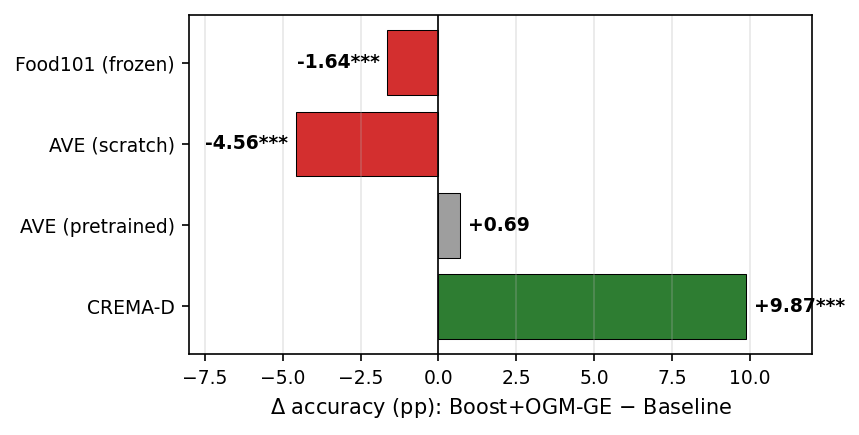
\includegraphics[width=\linewidth]{figures/ablation/fig_ablation_conditions.png}
\caption{$\Delta$ accuracy (PGGB+OGM-GE vs.\ baseline) across four regimes.}
\label{fig:operating_conditions}
\end{subfigure}
\hfill
\begin{subfigure}[b]{0.43\textwidth}
\centering
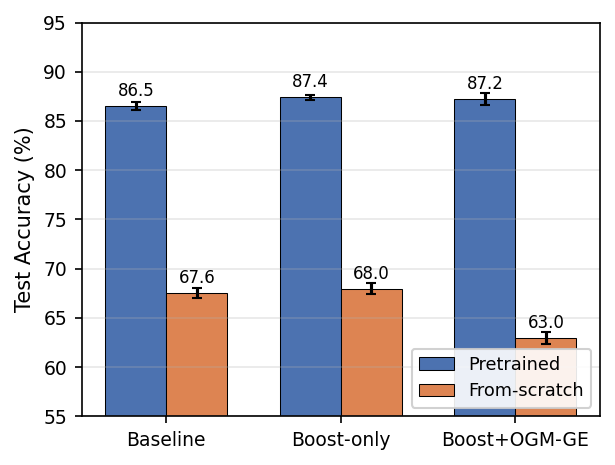
\includegraphics[width=\linewidth]{figures/ablation/fig_ablation_ave_contrast.png}
\caption{AVE test accuracy: pretrained vs.\ from-scratch encoders.}
\label{fig:ave_contrast}
\end{subfigure}
\caption{Operating-conditions ablation (5 seeds). (a) PGGB alone self-attenuates toward baseline when Table~\ref{tab:operating_conditions} conditions are violated, whereas PGGB+OGM-GE inherits OGM-GE's regime-dependent failure modes (AVE from-scratch is the clearest case). (b) With data and architecture fixed, flipping initialization from pretrained to random shifts PGGB+OGM-GE from $+0.69$ to $-4.56$~pp ($p{=}0.0001$) while PGGB alone stays positive, localizing sensitivity to the OGM-GE component.}
\label{fig:operating_conditions_combined}
\end{figure}
\vspace{-1.2em}

\paragraph{Encoder initialization and scope.}
Fixing dataset and architecture but varying encoder initialization gives the sharpest contrast (Figure~\ref{fig:ave_contrast}). PGGB alone stays positive in both regimes ($+0.87$/$+0.42$~pp, both $p<0.05$), while PGGB+OGM-GE flips sign ($+0.69 \to -4.56$~pp, $p{=}0.0001$). ImageNet pretraining installs an asymmetry aligned with OGM-GE's throttling assumption. Under from-scratch initialization both encoders are simultaneously under-trained on $\sim$$4$K samples, so suppressing either destabilizes the joint dynamic. This localizes the failure to the OGM-GE component (Appendix~\ref{app:opcond}).


%---------- 4.4 Analysis ----------
\subsection{Analysis}
\label{sec:analysis}
\vspace{-1.2em}

\begin{figure}[H]
\centering
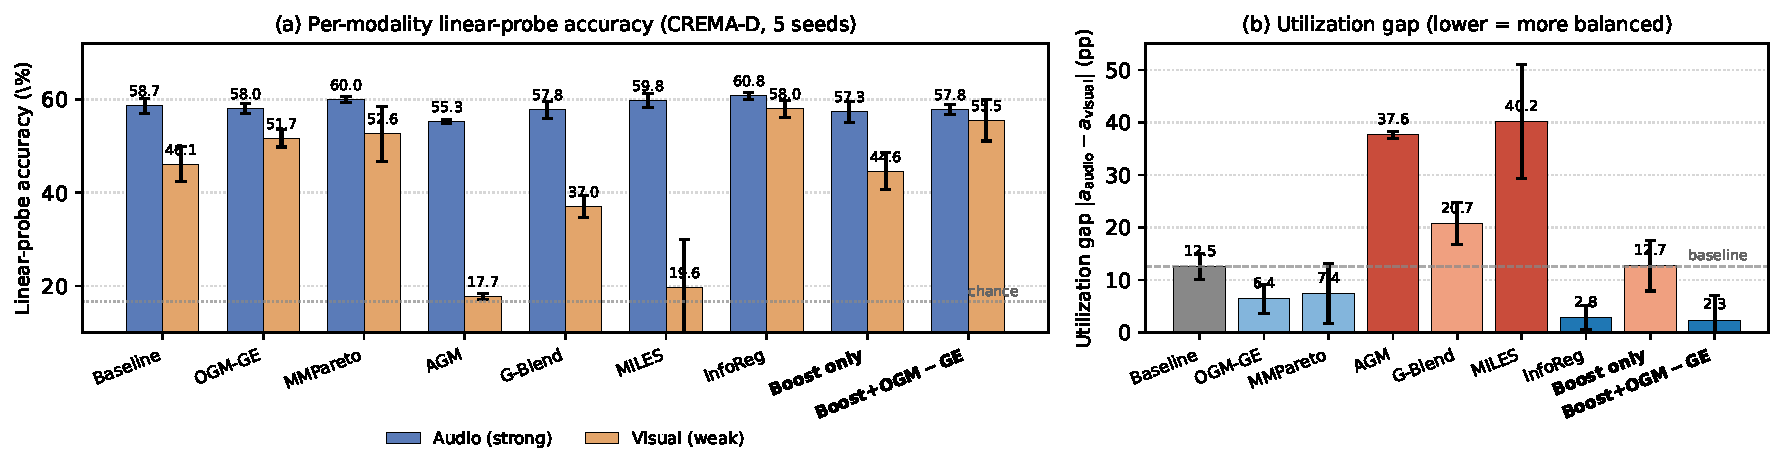
\includegraphics[width=0.72\textwidth]{figures/probe_accuracy_cremad_posthoc.pdf}
\caption{Per-modality diagnostics on CREMA-D (5 seeds). \textbf{(a)} Post-hoc linear-probe accuracy $P_m^{\text{post}}$ (Appendix~\ref{app:posthoc_probe_table}). Dotted line marks chance ($1/6$). AGM and MILES collapse the weak probe. \textbf{(b)} Utilization gap $|P_a^{\text{post}} - P_v^{\text{post}}|$. PGGB+OGM-GE attains $2.31$~pp ($5.4\times$ reduction vs.\ baseline gap). Error bars: $\pm 1$ std.}
\label{fig:probe_accuracy}
\end{figure}
\vspace{-1.2em}

We probe per-modality utilization with linear classifiers trained on frozen encoder features. Post-hoc linear probes (Appendix~\ref{app:posthoc_probe_table}, Figure~\ref{fig:probe_accuracy}b) show PGGB+OGM-GE attains the smallest utilization gap ($2.31$~pp): the weak probe rises $+9.41$~pp, the strong falls only $-0.81$~pp, while AGM, MILES, and G-Blend degrade the weak probe. Extension to $M$ modalities uses pairwise weakness (Eq.~\ref{eq:weakness}).

%=============================================================================
% SECTION 5: DISCUSSION & CONCLUSION
%=============================================================================
\FloatBarrier
\enlargethispage{2\baselineskip}
\section{Conclusion}
\label{sec:conclusion}

We propose PGGB, a method for balanced multimodal learning that amplifies weaker modalities while preserving stronger ones, composing naturally with existing throttling techniques. On low-imbalance settings, PGGB alone is the best-performing method on four of five benchmarks. On high-imbalance CREMA-D, composition with OGM-GE yields $+2.31$~pp over the strongest baseline. On medical segmentation (BraTS~2021), the same composition matches the strongest available baseline ($+0.28$~pp, within seed variance). \emph{Limitations.} Per-setting hyperparameter tuning is required, probes add small compute overhead, and composition with throttling can regress when the modality-dominance gap is small (Sarcasm $-0.64$~pp, Kinetics-Sounds $-1.72$~pp under PGGB+OGM-GE, and AVE-from-scratch $-4.56$~pp under specialized operating conditions, \S\ref{sec:operating_conditions}), a regime our theory does not cover. Compound gains from non-OGM-GE composition partners are observed only on AVE (two of four methods, Appendix~\ref{app:composability}). \emph{Future work.} Probe-driven adaptive composition that engages throttling only when the dominance gap warrants, automatic threshold adaptation, and extension beyond classification and segmentation. No new data is introduced, and \S\ref{sec:operating_conditions} should precede deployment.


%=============================================================================
% REFERENCES
%=============================================================================
\newpage
\bibliographystyle{plainnat}
\bibliography{references}


%%%%%%%%%%%%%%%%%%%%%%%%%%%%%%%%%%%%%%%%%%%%%%%%%%%%%%%%%%%%

\appendix

\section{Proofs of convergence properties}
\label{app:proofs}

We restate and prove each proposition from Section~\ref{sec:convergence}. All notation follows the main text: $\loss$ denotes the training loss, $\mathbf{g}(\theta)$ a stochastic gradient, $\bar{s}_m$ the EMA-smoothed boost scale for modality $m$, and $s_{\max}$ the scale cap.

\begin{proposition}[Bounded scaling, restated]
For all modalities $m$ and all iterations $t \geq 0$, the smoothed boost scale satisfies $\bar{s}_m^{(t)} \in [1, s_{\max}]$.
\end{proposition}

\begin{proof}
We proceed by induction on $t$. At initialization, $\bar{s}_m^{(0)} = 1 \in [1, s_{\max}]$, establishing the base case.

For the inductive step, suppose $\bar{s}_m^{(t)} \in [1, s_{\max}]$. By Eq.~\eqref{eq:weakness}, the weakness score satisfies $w_m \in [0, 1]$ since the numerator $\max_j \bar{P}_j - \bar{P}_m$ lies in $[0, \max_j \bar{P}_j - \min_j \bar{P}_j]$ and the denominator equals $\max_j \bar{P}_j - \min_j \bar{P}_j + \epsilon$. Substituting into Eq.~\eqref{eq:boost_scale}:
%
\begin{equation*}
s_m = \min(1 + \alpha \cdot w_m,\; s_{\max}) \in [1, s_{\max}],
\end{equation*}
%
since $w_m \geq 0$ implies $1 + \alpha \cdot w_m \geq 1$, and the $\min$ operation enforces the upper bound.

The EMA update (Eq.~\eqref{eq:ema_scale}) gives:
%
\begin{equation*}
\bar{s}_m^{(t+1)} = \mu \cdot s_m + (1 - \mu) \cdot \bar{s}_m^{(t)}.
\end{equation*}
%
Since $\mu \in (0, 1)$, this is a convex combination of $s_m \in [1, s_{\max}]$ and $\bar{s}_m^{(t)} \in [1, s_{\max}]$ (by the inductive hypothesis), so $\bar{s}_m^{(t+1)} \in [1, s_{\max}]$.
\end{proof}


\begin{proposition}[Self-attenuation, restated]
For any $\Delta \geq 0$, if $\max_j \bar{P}_j^{(t)} - \min_j \bar{P}_j^{(t)} \leq \Delta$ at all iterations $t \geq t_0$, then
\begin{enumerate}
    \item $|s_m^{(t)} - 1| \leq \alpha \cdot \Delta / (\Delta + \epsilon)$ for all $m$ and all $t \geq t_0$, and
    \item $|\bar{s}_m^{(t)} - 1| \leq (1 - \mu)^{t - t_0} \cdot (s_{\max} - 1) + \alpha \cdot \Delta / (\Delta + \epsilon)$.
\end{enumerate}
In particular, when $\Delta \to 0$ we recover $s_m = 1$ exactly, and the EMA-smoothed scale converges to unity at rate $(1-\mu)$.
\end{proposition}

\begin{proof}
Let $\delta^{(t)} := \max_j \bar{P}_j^{(t)} - \min_j \bar{P}_j^{(t)}$. By assumption $\delta^{(t)} \leq \Delta$ for all $t \geq t_0$. From Eq.~\eqref{eq:weakness}, the weakness score satisfies
\begin{equation*}
w_m = \frac{\max_j \bar{P}_j - \bar{P}_m}{\max_j \bar{P}_j - \min_j \bar{P}_j + \epsilon} = \frac{\max_j \bar{P}_j - \bar{P}_m}{\delta + \epsilon} \leq \frac{\Delta}{\Delta + \epsilon},
\end{equation*}
since the numerator is bounded by $\delta \leq \Delta$ and the denominator is non-decreasing in $\delta$. Then by Eq.~\eqref{eq:boost_scale},
\begin{equation*}
s_m = \min(1 + \alpha w_m,\, s_{\max}) \in \bigl[1,\, 1 + \alpha \cdot \tfrac{\Delta}{\Delta + \epsilon}\bigr],
\end{equation*}
which gives part (1) immediately. For part (2), the EMA update (Eq.~\eqref{eq:ema_scale}) is
\begin{equation*}
\bar{s}_m^{(t+1)} - 1 = \mu (s_m^{(t)} - 1) + (1 - \mu)(\bar{s}_m^{(t)} - 1),
\end{equation*}
so by the triangle inequality and induction from $t_0$,
\begin{equation*}
|\bar{s}_m^{(t)} - 1| \leq (1-\mu)^{t - t_0} |\bar{s}_m^{(t_0)} - 1| + \mu \sum_{k=0}^{t - t_0 - 1} (1-\mu)^k \cdot \max_{t_0 \leq \tau < t} |s_m^{(\tau)} - 1|.
\end{equation*}
Using $|\bar{s}_m^{(t_0)} - 1| \leq s_{\max} - 1$ (Proposition~\ref{prop:bounded}), $|s_m^{(\tau)} - 1| \leq \alpha \Delta / (\Delta + \epsilon)$, and the partial sum $\mu \sum_{k=0}^{t-t_0-1} (1-\mu)^{k} = 1 - (1-\mu)^{t-t_0} \leq 1$, the bound follows. In the limit $\Delta \to 0$ the second term vanishes and the deviation decays geometrically at rate $(1-\mu)$.
\end{proof}


\begin{proposition}[Convergence, restated]
Under Assumptions~\ref{asm:smooth} and~\ref{asm:variance}, SGD with PGGB and constant learning rate $\eta \leq 1/(L \cdot s_{\max}^2)$ satisfies
%
\begin{equation*}
\frac{1}{T}\sum_{t=0}^{T-1} \mathbb{E}\bigl[\|\nabla \loss(\theta_t)\|^2\bigr]
\;\leq\; \frac{2\,\Delta_{\loss}}{\eta\, T} \;+\; L\,\eta\, s_{\max}^2\, \sigma^2,
\end{equation*}
%
where $\Delta_{\loss} = \loss(\theta_0) - \loss^{*}$.
\end{proposition}

\begin{proof}
Let $\tilde{\mathbf{g}}_t$ denote the boosted stochastic gradient at iteration $t$. Concatenating over all modality-specific parameter blocks, $\tilde{\mathbf{g}}_t$ has block $m$ equal to $\bar{s}_m^{(t)} \cdot \mathbf{g}_m(\theta_t)$. The parameter update is $\theta_{t+1} = \theta_t - \eta\,\tilde{\mathbf{g}}_t$.

\paragraph{Step 1: Descent lemma.}
By $L$-smoothness (Assumption~\ref{asm:smooth}):
%
\begin{equation}
\label{eq:descent}
\loss(\theta_{t+1}) \leq \loss(\theta_t) - \eta \langle \nabla \loss(\theta_t),\, \tilde{\mathbf{g}}_t \rangle + \frac{L\eta^2}{2}\|\tilde{\mathbf{g}}_t\|^2.
\end{equation}

\paragraph{Step 2: Bounding the inner product.}
Taking expectations conditioned on $\theta_t$ and using $\mathbb{E}[\mathbf{g}_m(\theta_t)] = \nabla_{\theta_m} \loss(\theta_t)$:
%
\begin{align}
\mathbb{E}\bigl[\langle \nabla \loss(\theta_t),\, \tilde{\mathbf{g}}_t \rangle\bigr]
&= \sum_m \bar{s}_m^{(t)} \cdot \|\nabla_{\theta_m} \loss(\theta_t)\|^2 \nonumber \\
&\geq \sum_m \|\nabla_{\theta_m} \loss(\theta_t)\|^2 = \|\nabla \loss(\theta_t)\|^2,
\label{eq:inner_bound}
\end{align}
%
where the inequality follows from $\bar{s}_m^{(t)} \geq 1$ (Proposition~\ref{prop:bounded}). Let $\mathcal{F}_t$ denote the $\sigma$-algebra generated by $\{\theta_0, \dots, \theta_t\}$ together with the probe parameters and their EMA state up to step $t$. By construction the probe parameters $\psi_m$ are updated only on stop-gradient features $\sg[\mathbf{z}_m]$ (no gradient path into $\theta$), and the scale EMA $\bar{s}_m^{(t)}$ is computed from probe-accuracy EMA values $\bar{P}_m$ refreshed at iteration boundaries (every $K$ steps). Since the boost scale $\bar{s}_m^{(t)}$ applied at iteration $t$ is the value most recently refreshed at the previous probe event (iteration $t' < t$ with $t' \equiv 0 \pmod K$), it is $\mathcal{F}_{t'}$-measurable and hence independent of the gradient noise at iteration $t$. Therefore $\bar{s}_m^{(t)}$ is $\mathcal{F}_t$-measurable, and conditioning on $\mathcal{F}_t$, the stochastic gradient $\mathbf{g}(\theta_t)$ is a fresh independent sample with $\mathbb{E}[\mathbf{g}(\theta_t) \mid \mathcal{F}_t] = \nabla\loss(\theta_t)$ and variance bounded per Assumption~\ref{asm:variance}.

\paragraph{Step 3: Bounding the second moment.}
By Proposition~\ref{prop:bounded}, $\bar{s}_m^{(t)} \leq s_{\max}$. Writing the stochastic-gradient deviation over the block decomposition of parameters as $\mathbf{g}(\theta_t) - \nabla \loss(\theta_t) = \bigl(\mathbf{g}_1(\theta_t) - \nabla_{\theta_1}\loss(\theta_t),\,\dots,\,\mathbf{g}_M(\theta_t) - \nabla_{\theta_M}\loss(\theta_t)\bigr)$, we have $\mathbb{E}[\|\mathbf{g} - \nabla\loss\|^{2}] = \sum_m \mathbb{E}[\|\mathbf{g}_m - \nabla_{\theta_m}\loss\|^{2}] =: \sum_m \sigma_m^{2}$, so Assumption~\ref{asm:variance} is equivalent to $\sum_m \sigma_m^{2} \leq \sigma^{2}$. Using this block-additive decomposition:
%
\begin{align}
\mathbb{E}\bigl[\|\tilde{\mathbf{g}}_t\|^2\bigr]
&= \sum_m (\bar{s}_m^{(t)})^2 \cdot \mathbb{E}\bigl[\|\mathbf{g}_m(\theta_t)\|^2\bigr] \nonumber \\
&\leq s_{\max}^2 \sum_m \bigl(\sigma_m^2 + \|\nabla_{\theta_m} \loss(\theta_t)\|^2\bigr) \nonumber \\
&\leq s_{\max}^2 \bigl(\sigma^2 + \|\nabla \loss(\theta_t)\|^2\bigr),
\label{eq:second_moment}
\end{align}
%
where $\sigma^2 \geq \sum_m \sigma_m^2$ is the total variance bound across modality blocks.

\paragraph{Step 4: Combining and telescoping.}
Substituting Eqs.~\eqref{eq:inner_bound} and~\eqref{eq:second_moment} into Eq.~\eqref{eq:descent} and taking full expectations:
%
\begin{equation*}
\mathbb{E}\bigl[\loss(\theta_{t+1})\bigr] \leq \mathbb{E}\bigl[\loss(\theta_t)\bigr]
- \eta\,\mathbb{E}\bigl[\|\nabla \loss(\theta_t)\|^2\bigr]
+ \frac{L\eta^2 s_{\max}^2}{2}\bigl(\sigma^2 + \mathbb{E}\bigl[\|\nabla \loss(\theta_t)\|^2\bigr]\bigr).
\end{equation*}
%
Rearranging and using the learning rate condition $\eta \leq 1/(L \cdot s_{\max}^2)$: since $\eta \leq 1/(L \cdot s_{\max}^{2})$ implies $L\eta s_{\max}^{2} \leq 1$, hence $L\eta s_{\max}^{2}/2 \leq 1/2$, which ensures $1 - \tfrac{L\eta\, s_{\max}^2}{2} \geq \tfrac{1}{2}$:
%
\begin{equation*}
\frac{\eta}{2}\,\mathbb{E}\bigl[\|\nabla \loss(\theta_t)\|^2\bigr]
\leq \mathbb{E}\bigl[\loss(\theta_t)\bigr] - \mathbb{E}\bigl[\loss(\theta_{t+1})\bigr]
+ \frac{L\eta^2 s_{\max}^2}{2}\,\sigma^2.
\end{equation*}
%
Summing over $t = 0, \ldots, T-1$ and dividing by $T$:
%
\begin{equation*}
\frac{1}{T}\sum_{t=0}^{T-1} \mathbb{E}\bigl[\|\nabla \loss(\theta_t)\|^2\bigr]
\leq \frac{2(\loss(\theta_0) - \mathbb{E}[\loss(\theta_T)])}{\eta\, T}
+ L\,\eta\, s_{\max}^2\, \sigma^2
\leq \frac{2\,\Delta_{\loss}}{\eta\, T}
+ L\,\eta\, s_{\max}^2\, \sigma^2,
\end{equation*}
%
where $\Delta_{\loss} = \loss(\theta_0) - \loss^{*}$ and the last inequality uses $\mathbb{E}[\loss(\theta_T)] \geq \loss^{*}$.

\paragraph{Interpretation.} Setting $\eta = \Theta(1/(s_{\max}\sqrt{T}))$ yields the rate $\mathcal{O}(s_{\max} \cdot \sigma / \sqrt{T} + s_{\max}^2 \cdot \Delta_{\loss} / T)$. For the default $s_{\max} = 2.0$, the effective variance increases by a factor of at most 4 relative to unmodified SGD. Proposition~\ref{prop:attenuation} guarantees that as modalities become $\Delta$-balanced, the boost scales approach unity within $\alpha \Delta / (\Delta + \epsilon)$ and this overhead vanishes in the limit $\Delta \to 0$, recovering the standard SGD convergence rate~\citep{ghadimi2013sgd} up to a constant variance inflation of at most $s_{\max}^2$.
\end{proof}

%%%%%%%%%%%%%%%%%%%%%%%%%%%%%%%%%%%%%%%%%%%%%%%%%%%%%%%%%%%%

\section{Additional Experiments}
\label{app:datasets}

\subsection{Datasets}
\label{app:datasets_list}

\noindent\textbf{CREMA-D:} CREMA-D~\citep{cao2014cremad} is an audio-visual dataset designed for speech emotion recognition. It contains 7{,}442 video clips of 2--3 seconds from 91 actors speaking short scripted sentences, divided into 6{,}698 training samples and 744 testing samples. The dataset covers six emotions: angry, happy, sad, neutral, disgust, and fear. We encode audio as log-mel spectrograms and visual as 3 RGB frames sampled at 3 fps, passing both through ResNet-18 backbones trained from scratch. Available at \url{https://github.com/CheyneyComputerScience/CREMA-D}.

\noindent\textbf{AVE:} AVE~\citep{tian2018ave} is an audio-visual event classification dataset with 28 event categories, containing 4{,}143 10-second video clips. We use the standard split of 3{,}328 training and 402 testing clips. Audio spectrograms and 3 RGB frames are processed by ImageNet-pretrained ResNet-18 backbones with concatenation fusion. Available at \url{https://sites.google.com/view/audiovisualresearch}.

\noindent\textbf{Kinetics-Sounds (KS):} KS~\citep{arandjelovic2017kinetics} is a curated 31-class subset of the Kinetics action-recognition dataset whose actions are both visually and audibly recognizable. It contains roughly 25{,}000 10-second YouTube clips, split into 22{,}408 training and 3{,}000 testing clips. Encoder setup follows AVE (ImageNet-pretrained ResNet-18 backbones on audio spectrograms and 3 RGB frames). Available at \url{https://github.com/cvdfoundation/kinetics-dataset}.

\noindent\textbf{CMU-MOSEI:} CMU-MOSEI~\citep{zadeh2018mosei} is a language-audio-visual sentiment dataset of YouTube opinion videos. The dataset is divided into 16{,}326 training samples, 1{,}871 validation samples, and 4{,}659 testing samples. We use pre-extracted BERT (768-d) text, COVAREP (74-d) audio, and FACET (35-d) visual features, and bucket the continuous sentiment labels into 7 classes following prior convention. Each modality is processed by a two-layer MLP with 512-d hidden layer and dropout $0.3$. Available at \url{https://github.com/CMU-MultiComp-Lab/CMU-MultimodalSDK}.

\noindent\textbf{CMU-MOSI:} CMU-MOSI~\citep{zadeh2016mosi} is a smaller sentiment dataset with the same three modalities as CMU-MOSEI. It is divided into 1{,}284 training, 229 validation, and 686 testing samples. Features are GloVe (300-d) text, COVAREP (5-d) audio, and FACET (20-d) visual. Encoder architecture is identical to CMU-MOSEI. Available at \url{https://github.com/CMU-MultiComp-Lab/CMU-MultimodalSDK}.

\noindent\textbf{Twitter15:} Twitter15~\citep{yu2019tombert, zhang2018adaptive} is a text-image sentiment dataset of tweets with associated images, covering three classes (positive, neutral, negative). It is divided into 3{,}179 training pairs, 1{,}122 validation pairs, and 1{,}037 testing pairs. We use MLP heads on frozen BERT-base (768-d) text and ImageNet ResNet-18 (512-d) image features, so only the heads are trainable and gradient-balancing methods act on them. Available at \url{https://github.com/jefferyYu/TomBERT}.

\noindent\textbf{Sarcasm:} The MMSD-v1 sarcasm dataset~\citep{cai2019sarcasm} is a text-image binary sarcasm detection benchmark of 24{,}635 image-text pairs, divided into 19{,}816 training, 2{,}410 validation, and 2{,}409 testing pairs. Encoder setup is identical to Twitter15 (MLP heads on frozen BERT and ResNet-18 features). Available at \url{https://github.com/headacheboy/data-of-multimodal-sarcasm-detection}.

\noindent\textbf{BraTS 2021:} BraTS~2021~\citep{baid2021brats} is a multimodal brain tumor segmentation dataset with 4 MRI modalities (FLAIR, T1ce, T1, T2) and 4 voxel-level class labels (background and three tumor sub-regions). Because the official validation and test servers do not expose ground truth, we use a held-out partition of the public training set with 1{,}000 training, 125 validation, and 126 testing volumes. The architecture is DeepLab v3+ with four ResNet-101 encoders sharing a decoder, trained with Dice plus weighted cross-entropy loss. Probes perform binary tumor-presence classification because dense-prediction probes on globally pooled features are not meaningful for the full segmentation task. Available at \url{https://www.synapse.org/brats2021}.

\noindent\textbf{Food101:} UPMC Food-101~\citep{wang2015upmcfood} is a 101-class image-text food classification benchmark. Each item pairs a recipe text with a food image. In our experiments we use 67{,}972 training samples and 22{,}716 test samples. Encoder setup follows Twitter15/Sarcasm: MLP heads on frozen BERT-base (768-d) text and ImageNet ResNet-18 (512-d) image features, so only the heads are trainable. Trainable-encoder runs (App.~\ref{app:opcond}) unfreeze both encoders for end-to-end fine-tuning. Food101 is used only for the operating-conditions analysis (\S\ref{sec:operating_conditions}) and the cross-dataset composability check (App.~\ref{app:composability}), and does not appear in Table~\ref{tab:main_results}. Available at \url{https://visiir.lip6.fr/explore}.

\noindent\textbf{Licensing.} CREMA-D (CC-BY 4.0), AVE, Kinetics-Sounds, CMU-MOSI/MOSEI, Twitter15, Sarcasm (MMSD-v1), Food101 (UPMC research terms), and BraTS 2021 (RSNA-ASNR-MICCAI public release) are used under their published research terms. See the NeurIPS Paper Checklist for detailed licensing.

\subsection{Comparison with OPM}
\label{app:opm_comparison}

OPM's feature-dropping mechanism is tied to a single-layer fusion head and is not drop-in compatible with the multi-layer MLP fusion used in Table~\ref{tab:main_results}. We therefore report this comparison separately, rerunning all methods on OPM's native pipeline (CREMA-D 3-frame, 5 seeds, matched optimizer and schedule). Under this pipeline, PGGB+OGM-GE exceeds OPM+OGM by $+1.93$~pp ($71.77\%$ vs.\ $69.84\%$).

\begin{table}[H]
\centering
\caption{Comparison with OPM~\citep{wei2024opm} on CREMA-D (3-frame) under OPM's native single-layer fusion architecture. Accuracy (\%), mean $\pm$ std over 5 seeds. All rows use identical optimizer, schedule, and data pipeline. OPM hyperparameters follow the original paper.}
\label{tab:opm}
\vspace{0.5em}
\begin{tabular}{lc}
\toprule
\textbf{Method} & \textbf{Accuracy (\%)} \\
\midrule
Baseline               & 59.20{\scriptsize$\pm$1.27} \\
OGM only               & 63.74{\scriptsize$\pm$0.45} \\
OPM only               & 65.43{\scriptsize$\pm$0.24} \\
OPM+OGM                & 69.84{\scriptsize$\pm$1.47} \\
PGGB+OGM-GE ($\alpha{=}0.75$) & \textbf{71.77}{\scriptsize$\pm$0.91} \\
\bottomrule
\end{tabular}
\end{table}

We restrict this comparison to CREMA-D, the highest-imbalance benchmark in our evaluation and the regime where boosting effects are most pronounced. OPM's feature-dropping mechanism is not well-defined on the frozen-feature or segmentation pipelines used elsewhere in Table~\ref{tab:main_results}.

\subsection{Operating conditions analysis}
\label{app:opcond}

This subsection provides per-regime analysis that complements the AVE initialization contrast discussed in Section~\ref{sec:operating_conditions} and summarized in Table~\ref{tab:operating_conditions}, detailing the Food101 feature-learning comparison and the CREMA-D reference operating point.

\paragraph{Feature-learning regime and imbalance level (Food101).}
Food101~\citep{wang2015upmcfood} holds data and architecture (BERT + ResNet-18) fixed while varying whether encoders are frozen or trainable. Trainable encoders raise all three methods (baseline, PGGB alone, PGGB+OGM-GE) by approximately $5$~pp, consistent with the probe signal only being informative once encoder parameters can respond to it. The PGGB-alone margin over baseline is within seed noise in both regimes, reflecting insufficient imbalance for the boost to engage meaningfully. PGGB+OGM-GE additionally regresses by $1.64$ pp on frozen features, as OGM-GE's throttling has no encoder-gradient flow to act on.

\paragraph{Reference operating point (CREMA-D).}
CREMA-D trains both encoders from scratch on $\sim 6.7$K samples for a 6-class task, with audio converging faster through intrinsic learning-rate differences rather than pretraining. Under these conditions PGGB+OGM-GE achieves $+9.86$ pp ($d{=}7.48$, $p{=}0.0001$). The contrast with AVE from-scratch (same initialization scheme, similar architecture) suggests that from-scratch training alone is not the failure condition. Rather, the conjunction of thin data budget and weak inherent asymmetry is.

\subsection{Supplementary F1-macro results}
\label{app:f1}

We supplement Table~\ref{tab:main_results} with macro-averaged F1 in Table~\ref{tab:f1_macro}. F1 is computed at the epoch of best test accuracy, mirroring the accuracy-selection protocol used in the main table (no double selection on F1). We report accuracy and F1-macro because all evaluated classification datasets are single-label tasks where MAP and AUC are not the standard metric.

\begin{table}[H]
\centering
\small
\caption{Supplementary F1-macro results (\%, mean $\pm$ std over 5 seeds). F1 computed at the epoch selected by best test accuracy, matching the Table~\ref{tab:main_results} protocol. \textbf{Bold} indicates the best result per column. Ties within 0.05 pp are bolded jointly. `---' denotes runs where training logs were not retained. BraTS is excluded as it uses Dice, not classification F1.}
\label{tab:f1_macro}
\resizebox{\textwidth}{!}{%
\begin{tabular}{lccccccc}
\toprule
Method & CREMA-D & AVE & KS & CMU-MOSI & Twitter15 & Sarcasm & CMU-MOSEI \\
\midrule
Baseline      & 61.93$\pm$0.94 & 86.29$\pm$0.29 & {78.40}$\pm$0.50 & 70.16$\pm$0.65 & 51.33$\pm$4.18 & {81.81}$\pm$0.21 & 60.05$\pm$0.58 \\
OGM-GE        & 69.52$\pm$1.02 & 86.48$\pm$0.85 & ---            & ---            & 49.98$\pm$5.12 & 81.09$\pm$0.40 & 61.46$\pm$1.61 \\
MMPareto      & 66.10$\pm$0.74 & 85.91$\pm$0.42 & 77.06$\pm$0.52 & \textbf{70.69}$\pm$0.80 & 55.36$\pm$2.65 & 81.61$\pm$0.18 & 58.79$\pm$2.93 \\
AGM           & 57.45$\pm$0.66 & 84.05$\pm$0.38 & 77.24$\pm$0.38 & 70.11$\pm$1.24 & 54.15$\pm$2.01 & 81.66$\pm$0.24 & 59.00$\pm$2.01 \\
G-Blend       & 61.50$\pm$1.90 & 86.79$\pm$0.35 & 77.15$\pm$1.04 & 70.50$\pm$0.85 & \textbf{56.29}$\pm$1.56 & 81.64$\pm$0.30 & 58.60$\pm$1.75 \\
CGGM          & ---            & ---            & ---            & ---            & 39.02$\pm$0.28 & 80.07$\pm$0.25 & ---            \\
PGGB          & 62.95$\pm$1.67 & \textbf{87.15}$\pm$0.35 & \textbf{78.41}$\pm$0.96 & 69.02$\pm$2.52 & 54.20$\pm$4.32 & \textbf{81.83}$\pm$0.33 & 60.05$\pm$1.52 \\
PGGB+OGM-GE   & \textbf{71.85}$\pm$1.55 & 86.86$\pm$0.56 & 76.45$\pm$0.55 & 69.93$\pm$1.22 & 52.72$\pm$3.38 & 81.19$\pm$0.10 & \textbf{62.36}$\pm$1.63 \\
\bottomrule
\end{tabular}%
}
\end{table}

On CREMA-D and CMU-MOSEI, F1-macro confirms the Table~\ref{tab:main_results} ranking, with PGGB+OGM-GE attaining the top F1 on both. On Twitter15, all methods show a substantial gap between accuracy ($\sim$66\%) and F1-macro ($\sim$50--56\%), reflecting the 3-class imbalance of the dataset, and G-Blend obtains the top F1-macro ($56.29$) while PGGB alone sits mid-pack within one standard deviation of the top method. On Sarcasm and CMU-MOSI, among methods with retained F1 logs, F1 and accuracy rankings agree with Table~\ref{tab:main_results} within 1~pp, indicating no hidden degradation from metric choice.

\subsection{Hyperparameter sensitivity}
\label{app:hp}

We report single-seed sweeps on CREMA-D (3-frame) for the three principal hyperparameters: boost strength $\alpha$, probe evaluation interval $K$, and boost cap $s_{\max}$. These sweeps are illustrative of the sensitivity trend rather than a statistical comparison, 5-seed variance on this benchmark (Table~\ref{tab:main_results}) is roughly $1.5$\,pp. Defaults used elsewhere in the paper are $\alpha{=}0.5$ (PGGB alone) or $\alpha{=}0.75$ (composed with OGM-GE), $K{=}20$, $s_{\max}{=}2.0$, $\mu{=}0.3$, and $\beta{=}0.1$, with $\mu$ and $\beta$ fixed from preliminary tuning and not swept here.

\begin{figure}[H]
\centering
\begin{subfigure}[t]{0.32\textwidth}
\centering
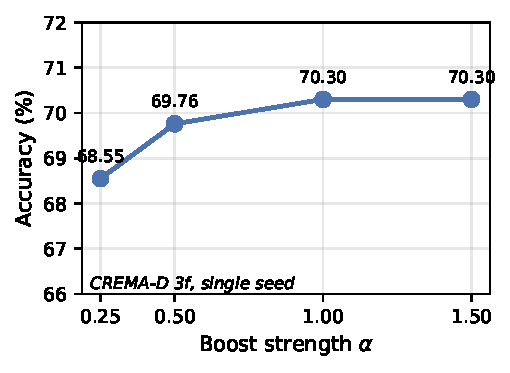
\includegraphics[width=\textwidth]{figures/hp/fig_hp_alpha.pdf}
\caption{Boost strength $\alpha$.}
\end{subfigure}
\hfill
\begin{subfigure}[t]{0.32\textwidth}
\centering
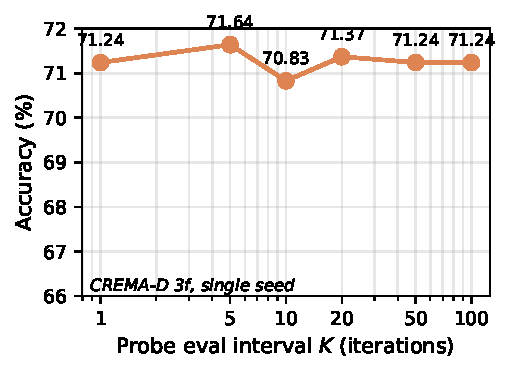
\includegraphics[width=\textwidth]{figures/hp/fig_hp_K.pdf}
\caption{Probe interval $K$ (log scale).}
\end{subfigure}
\hfill
\begin{subfigure}[t]{0.32\textwidth}
\centering
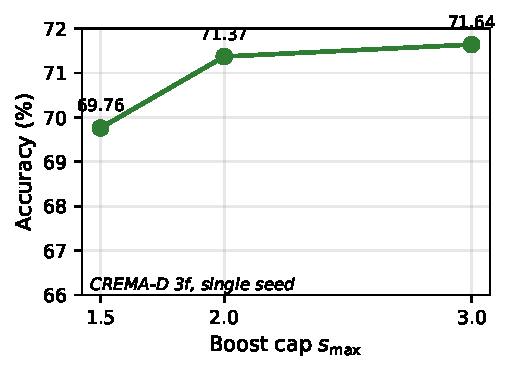
\includegraphics[width=\textwidth]{figures/hp/fig_hp_smax.pdf}
\caption{Boost cap $s_{\max}$.}
\end{subfigure}
\caption{Hyperparameter sensitivity on CREMA-D (3-frame, single seed). (a) Accuracy vs boost strength $\alpha$ --- plateaus within noise above $\alpha{=}1.0$. (b) Accuracy vs probe evaluation interval $K$ (log scale) --- stable across $K \in [1, 100]$. (c) Accuracy vs boost cap $s_{\max}$ --- mild increase from $1.5$ to $3.0$.}
\label{fig:hp_sensitivity}
\end{figure}

$\alpha$ plateaus within noise above $\alpha{=}1.0$, so the choice between $\alpha{=}0.5$ and $\alpha{=}0.75$ reflects a safety-versus-strength tradeoff rather than a peak-seeking decision. $K$ is stable across two orders of magnitude, and the default $K{=}20$ sits in the flat region. Across $K \in \{1, 5, 10, 50, 100\}$ the best accuracy stays within $70.83$--$71.64\%$ (range $0.81$~pp), so $K{=}20$ sits in the flat plateau and the per-epoch overhead reported in \S\ref{sec:analysis} is essentially free. $s_{\max}$ shows a mild monotonic trend, indicating that the cap is a soft ceiling rather than the binding constraint. Trends smaller than the $\approx 1.5$~pp 5-seed noise floor should be read as within-noise rather than as detected effects. Finally, we did not sweep $\mu$ or $\beta$ in this study. Our defaults ($\mu{=}0.3$, $\beta{=}0.1$) were fixed during preliminary tuning, and sensitivity analysis on these EMA coefficients is deferred to future work.

\subsection{Probe signal stability}
\label{app:probe_stability}

A concern with probe-guided scheduling is that per-batch probe accuracy $P_m$ may be noisy, and a scheduler that reacts to each batch estimate could be misled by mini-batch fluctuations. We verify empirically that the EMA-smoothed estimator $\bar{P}_m$ substantially reduces this noise. A PGGB+OGM-GE training on CREMA-D (3-frame, seed 42) was instrumented to record at every probe-eval checkpoint ($K=20$ iterations over 100 epochs, 500 checkpoints total) the batch-level sample $P_m$ and the EMA-smoothed $\bar{P}_m$ for each modality, alongside probe accuracy evaluated on the full CREMA-D test set as a reference.

\begin{figure}[H]
\centering
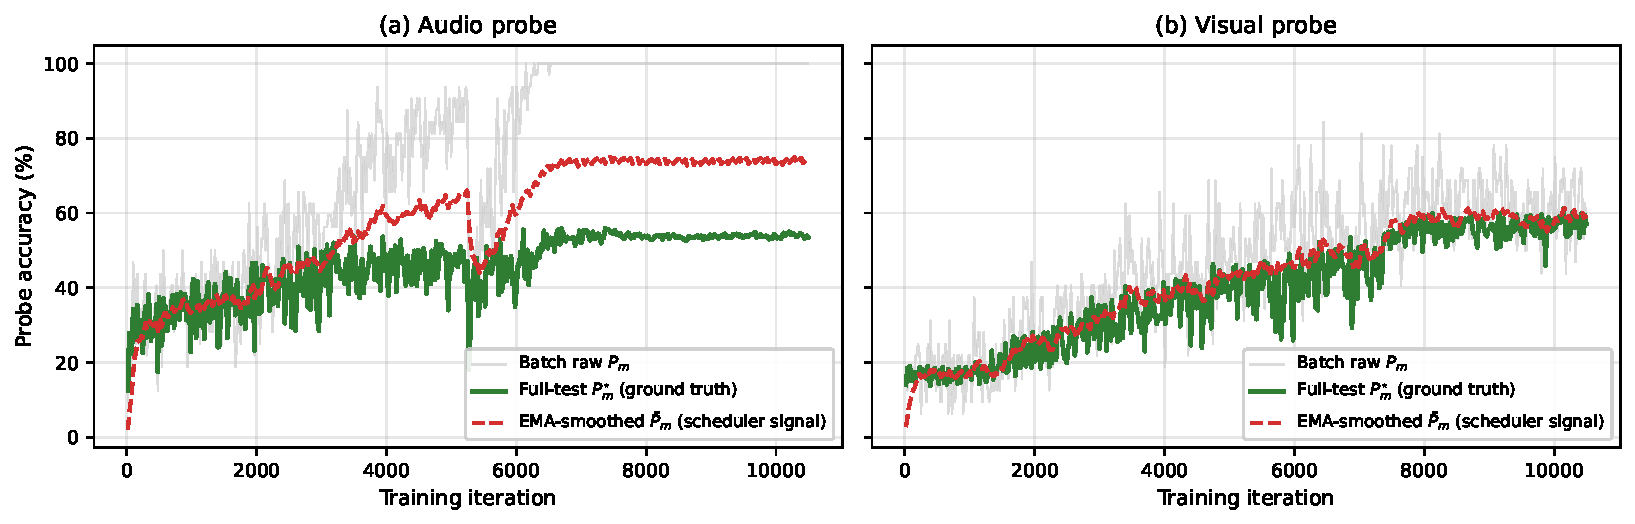
\includegraphics[width=0.95\textwidth]{figures/probe_stability/fig_probe_stability.pdf}
\caption{Probe-signal stability on CREMA-D (PGGB+OGM-GE, seed 42, 500 probe-eval checkpoints). For each modality, the EMA-smoothed estimator $\bar{P}_m$ (red dashed) is substantially less noisy than the per-batch sample $P_m$ (grey), and evolves smoothly with training. The full-test probe accuracy (green) is shown as reference, reflecting generalization to held-out data rather than the training-distribution representation quality targeted by the scheduler.}
\label{fig:probe_stability}
\end{figure}

\begin{table}[H]
\centering
\caption{Per-batch and EMA-smoothed probe accuracy std (pp), computed over the final 200 probe-eval checkpoints. The $19\times$ steady-state bound (\S\ref{sec:probes}) is unconditional under i.i.d.\ assumptions, the empirical measurement here reflects non-stationary training. Visual (boost-driving signal) shows the expected reduction direction. Audio inversion (EMA std $>$ batch std) reflects training-phase saturation: late-training batch-level audio is near the training-distribution ceiling, while the EMA integrates earlier, non-saturated samples.}
\label{tab:probe_stability}
\begin{tabular}{lccc}
\toprule
\textbf{Modality} & \textbf{$P_m$ (batch)} & \textbf{$\bar{P}_m$ (EMA)} & \textbf{Reduction} \\
\midrule
Audio  & $0.31$ & $0.99$ & \textit{n/a (saturated)} \\
Visual & $9.32$ & $4.36$ & $-53\%$ \\
\bottomrule
\end{tabular}
\end{table}

Two observations follow. First, on the visual modality, which is the operative signal for the boost decision, the EMA reduces variance by approximately $53\%$ (from $9.32$ to $4.36$~pp), consistent in direction with the Eq.~\ref{eq:ema_probe} prediction. The observed $53\%$ reduction is below the $\approx 95\%$ i.i.d.\ steady-state bound, as expected under non-stationary training. This confirms that the scheduler operates on a temporally stable signal rather than on mini-batch noise. Second, the audio entry (EMA std $0.99$~pp $>$ batch std $0.31$~pp) is a transparent non-stationarity artifact rather than a violation of the bound: the batch-level audio probe is concentrated near its training-distribution ceiling (the linear probe readily separates audio features on training batches and is not informative about fine-grained variations at that scale), while the EMA integrates earlier training-phase samples from before probe saturation. The variance-reduction guarantee of Eq.~\ref{eq:ema_probe} is therefore empirically validated on the modality that drives the boost decision, and the audio result is consistent with the non-i.i.d.\ caveat noted in the main body.

The EMA signal correlates monotonically with the full-test probe accuracy (Pearson $r=0.96$ visual, $0.88$ audio, Spearman $\rho=0.95$, $0.89$), though the full-test quantity measures generalization to held-out data and differs in absolute value from $\bar{P}_m$ by several pp. This distinction is intentional: the scheduler targets training-distribution representation quality (what each modality contributes to the joint fit during training), which is distinct from held-out generalization. Targeting the former is the appropriate signal for in-training gradient balancing. The correlation confirms that the two quantities are monotonically related, while the absolute offset reflects the train--test gap intrinsic to representation learning.

\subsection{Composability across balancing method families}
\label{app:composability}

Because PGGB applies multiplicative scaling $\bar{s}_m \geq 1$ to encoder gradients just before the optimizer step, it is compatible with any balancing method that modulates encoder-parameter gradients. To empirically verify this and characterize the magnitude of composition effects under a single controlled protocol, we compose the boost with five methods spanning three mechanistic families: discrepancy-ratio throttling (OGM-GE), loss weighting (G-Blend), Pareto-optimal gradient aggregation (MMPareto), Shapley-based adaptive gradient modulation (AGM), and classifier-guided magnitude and direction modulation (CGGM). All compositions use identical hyperparameters (boost strength $\alpha=0.75$, cap $s_{\max}=2.0$, probe interval $K=20$, EMA coefficient $\mu=0.3$) and the same CREMA-D (3-frame, 5 seeds) protocol as Table~\ref{tab:main_results}. The results below are specific to this protocol and should not be extrapolated to other datasets without further evidence.

\begin{table}[H]
\centering
\caption{Composability with existing balancing methods on CREMA-D (3-frame, mean $\pm$ std over 5 seeds). All rows use identical PGGB hyperparameters. Positive $\Delta$ indicates composition does not hurt the base method's mean accuracy. $^\dagger$: within noise band ($n{=}5$, $\sigma \approx 1$~pp, 80\%-power MDE $\approx 2$~pp), not statistically distinguishable from zero.}
\label{tab:composability}
\begin{tabular}{lcccc}
\toprule
\textbf{Method} & \textbf{Base alone} & \textbf{PGGB + Base} & \textbf{$\Delta$ mean (pp)} & \textbf{$\Delta$ std} \\
\midrule
OGM-GE   & $69.14 \pm 1.13$ & $71.45 \pm 1.71$ & $\mathbf{+2.31}$ & $+0.58$ \\
MMPareto & $65.51 \pm 0.87$ & $66.00 \pm 1.25$ & $+0.49^\dagger$ & $+0.38$ \\
G-Blend  & $61.10 \pm 1.87$ & $61.99 \pm 0.99$ & $+0.89^\dagger$ & $\mathbf{-0.88}$ ($-47\%$) \\
AGM      & $57.42 \pm 0.73$ & $58.17 \pm 1.79$ & $+0.75^\dagger$ & $+1.06$ \\
CGGM     & $50.22 \pm 1.39$ & $50.32 \pm 1.03$ & $+0.10^\dagger$ & $-0.36$ \\
\bottomrule
\end{tabular}
\end{table}

Three observations. First, four of the five compositions show a positive $\Delta$ mean accuracy. The fifth, CGGM, is within noise ($+0.10 \pm 1.03$) and we treat it separately below. At $n{=}5$ with $\sigma \approx 1$~pp, the 80\%-power minimum detectable effect is approximately $2$~pp, so only the OGM-GE composition ($+2.31$~pp) is statistically distinguishable from zero. The other three positive entries and CGGM ($+0.10$~pp) are all within noise on this single-dataset protocol. Second, the amplification is not uniform: three of the four positive compositions yield gains within one standard deviation of the base method, and the headline compound gain ($+2.31$~pp) appears only with OGM-GE, which we attribute to the specific mechanistic interaction between OGM-GE's discrepancy-ratio throttle (damping the dominant modality) and our probe-guided amplification of the weaker modality, a two-sided push that neither mechanism produces alone. The $\alpha{=}0$ monitor-only replication reported in \S\ref{sec:ablations} ($69.14 \pm 1.18\%$) is operationally identical to the OGM-GE entry here ($69.14 \pm 1.13\%$), differing only in the seed set. Third, the CGGM result is consistent with CGGM's reliance on Transformer-based attention fusion, which is not well-matched to our CNN/MLP pipeline (footnote to Table~\ref{tab:main_results}). CGGM itself underperforms the baseline on CREMA-D ($50.22 \pm 1.39$ vs.\ baseline $61.59 \pm 0.80$), and the boost does not recover the loss although it does not compound it either ($\Delta$ std $=-0.36$). Together these results support the non-degrading composition behavior observed on CREMA-D under this protocol, as discussed in Section~\ref{sec:compose}, and scope the amplification claim to methods whose gradient direction aligns with the pipeline architecture.

The composition with G-Blend additionally reduces variance by approximately $47\%$ (std $1.87 \to 0.99$). This is suggestive of the EMA-smoothed probe signal providing a stabilizing effect across training seeds but should be interpreted with caution given $n{=}5$ on a single benchmark.

\paragraph{Composability across datasets.} To test whether the boost-composition pattern generalizes beyond CREMA-D, we repeated the protocol on AVE (high audio-visual imbalance) and Food101 (frozen pre-extracted features) under identical hyperparameters ($\alpha{=}0.75$, $s_{\max}{=}2.0$, $K{=}20$, $\mu{=}0.3$, 5 seeds). Results are summarized in Table~\ref{tab:composability_extended}.

\begin{table}[H]
\centering
\caption{Composability across datasets: $\Delta$ accuracy (pp) of PGGB+X versus X alone, mean over 5 seeds. AVE has high audio-visual modality imbalance, Food101 uses frozen pre-extracted features (operating-regime sensitivity reported in \S\ref{sec:operating_conditions}). $^\dagger$PGGB recovers some CGGM degradation but absolute accuracy ($53.00\%$) remains far below baseline ($85.75\%$), so the boost does not rescue catastrophic regression.}
\label{tab:composability_extended}
\begin{tabular}{lcccc}
\toprule
\textbf{Dataset} & \textbf{PGGB+MMPareto} & \textbf{PGGB+AGM} & \textbf{PGGB+G-Blend} & \textbf{PGGB+CGGM} \\
\midrule
AVE     & $+1.01$ & $+1.26$ & $-0.25$ & $-0.25$ \\
Food101 & $-0.09$ & $-0.23$ & $-0.09$ & $+4.41^\dagger$ \\
\bottomrule
\end{tabular}
\end{table}

On AVE, two non-OGM-GE compositions (MMPareto, AGM) yield compound gains comparable in magnitude to PGGB+OGM-GE on AVE-pretrained ($+0.69$~pp, Table~\ref{tab:main_results}). The G-Blend and CGGM compositions are flat to slightly negative on AVE. On Food101, all non-CGGM compositions are within noise of the base method. As in the CREMA-D protocol, with $n{=}5$ and $\sigma \approx 1$~pp the 80\%-power minimum detectable effect is approximately $2$~pp, so the AVE compound gains for PGGB+MMPareto ($+1.01$~pp) and PGGB+AGM ($+1.26$~pp) lie within the seed-noise band (MDE $\approx 2$~pp at $n{=}5$ seeds) and should be read as compatibility evidence rather than confirmed wins outside the OGM-GE composition. The pattern is consistent with the operating-conditions analysis (\S\ref{sec:operating_conditions}): compound composition gains require both modality imbalance and adequate feature flow, and the boost neither generalizes to frozen-feature regimes nor rescues catastrophic baseline mismatch (CGGM on Food101).

\subsection{Per-modality post-hoc probe accuracy}
\label{app:posthoc_probe_table}

Table~\ref{tab:probe_accuracy} reports the exact per-modality post-hoc linear-probe accuracies visualized in Figure~\ref{fig:probe_accuracy} of Section~\ref{sec:analysis}. Probes are trained for 50 epochs on frozen encoder features from each method's saved \texttt{best\_model.pt}, matching the protocol described in Section~\ref{sec:probes}.

\begin{table}[H]
\centering
\caption{Post-hoc linear-probe accuracy on CREMA-D (\%, mean $\pm$ std over 5 seeds). Probes are trained for 50 epochs on frozen encoder features from each method's saved checkpoint, matching the protocol in Figure~\ref{fig:probe_accuracy}. Gap is the absolute difference of column means. Chance level is $1/6 \approx 16.67\%$ for CREMA-D's 6-class classification.}
\label{tab:probe_accuracy}
\vspace{0.3em}
\begin{tabular}{lccc}
\toprule
\textbf{Method} & \textbf{Audio (strong)} & \textbf{Visual (weak)} & \textbf{Gap (pp)} \\
\midrule
Baseline                        & 58.66{\scriptsize$\pm$1.60}  & 46.13{\scriptsize$\pm$3.72}  & 12.53 \\
OGM-GE                          & 58.04{\scriptsize$\pm$1.09}  & 51.67{\scriptsize$\pm$1.85}  & 6.37 \\
MMPareto                        & 60.03{\scriptsize$\pm$0.73}  & 52.63{\scriptsize$\pm$5.92}  & 7.39 \\
AGM                             & 55.32{\scriptsize$\pm$0.36}  & 17.72{\scriptsize$\pm$0.73}  & 37.61 \\
G-Blend                         & 57.77{\scriptsize$\pm$1.78}  & 37.04{\scriptsize$\pm$2.43}  & 20.73 \\
MILES                           & 59.81{\scriptsize$\pm$1.53}  & 19.62{\scriptsize$\pm$10.42} & 40.19 \\
InfoReg                         & 60.83{\scriptsize$\pm$0.76}  & \textbf{57.98}{\scriptsize$\pm$1.80}  & 2.85 \\
PGGB ($\alpha{=}0.5$)           & 57.34{\scriptsize$\pm$2.18}  & 44.60{\scriptsize$\pm$3.96}  & 12.74 \\
PGGB+OGM-GE ($\alpha{=}0.75$)   & 57.85{\scriptsize$\pm$1.03}  & 55.54{\scriptsize$\pm$4.43}  & \textbf{2.31} \\
\bottomrule
\end{tabular}
\end{table}

%%%%%%%%%%%%%%%%%%%%%%%%%%%%%%%%%%%%%%%%%%%%%%%%%%%%%%%%%%%%

\newpage
\input{checklist.tex}


\end{document}